%%%%%%%%%%%%%%%%%%%%%%%%%%%%%%%%%%%%%%%%%
% Masters/Doctoral Thesis 
% LaTeX Template
% Version 2.4 (22/11/16)
%
% This template has been downloaded from:
% http://www.LaTeXTemplates.com
%
% Version 2.x major modifications by:
% Vel (vel@latextemplates.com)
%
% This template is based on a template by:
% Steve Gunn (http://users.ecs.soton.ac.uk/srg/softwaretools/document/templates/)
% Sunil Patel (http://www.sunilpatel.co.uk/thesis-template/)
%
% Template license:
% CC BY-NC-SA 3.0 (http://creativecommons.org/licenses/by-nc-sa/3.0/)
%
%%%%%%%%%%%%%%%%%%%%%%%%%%%%%%%%%%%%%%%%%

%----------------------------------------------------------------------------------------
%	PACKAGES AND OTHER DOCUMENT CONFIGURATIONS
%----------------------------------------------------------------------------------------
\documentclass[
11pt, % The default document font size, options: 10pt, 11pt, 12pt
%oneside, % Two side (alternating margins) for binding by default, uncomment to switch to one side
spanish, % ngerman for German
singlespacing, % Single line spacing, alternatives: onehalfspacing or doublespacing
%draft, % Uncomment to enable draft mode (no pictures, no links, overfull hboxes indicated)
%nolistspacing, % If the document is onehalfspacing or doublespacing, uncomment this to set spacing in lists to single
%liststotoc, % Uncomment to add the list of figures/tables/etc to the table of contents
%toctotoc, % Uncomment to add the main table of contents to the table of contents
%parskip, % Uncomment to add space between paragraphs
%nohyperref, % Uncomment to not load the hyperref package
headsepline, % Uncomment to get a line under the header
%chapterinoneline, % Uncomment to place the chapter title next to the number on one line
%consistentlayout, % Uncomment to change the layout of the declaration, abstract and acknowledgements pages to match the default layout
]{MastersDoctoralThesis} % The class file specifying the document structure
\usepackage[utf8]{inputenc} % Required for inputting international characters
\usepackage{pdfpages}
\usepackage[T1]{fontenc} % Output font encoding for international characters
 
\usepackage{booktabs}
\newcommand{\tabitem}{~~\llap{\textbullet}~~}

\usepackage{palatino} % Use the Palatino font by default

\usepackage{placeins} %FloatBarrier

\usepackage[backend=bibtex,style=numeric,natbib=true]{biblatex} % Use the bibtex backend with the authoryear citation style (which resembles APA)

\addbibresource{Bibliografia.bib} % The filename of the bibliography

\usepackage[autostyle=true]{csquotes} % Required to generate language-dependent quotes in the bibliography

\usepackage{afterpage}

\newcommand\blankpage{%
    \null
    \thispagestyle{empty}%
    \addtocounter{page}{-1}%
    \newpage}
%----------------------------------------------------------------------------------------
%	MARGIN SETTINGS
%----------------------------------------------------------------------------------------

\geometry{
	paper=a4paper, % Change to letterpaper for US letter
	inner=2.5cm, % Inner margin
	outer=3.8cm, % Outer margin
	bindingoffset=.5cm, % Binding offset
	top=1.5cm, % Top margin
	bottom=1.5cm, % Bottom margin
	%showframe, % Uncomment to show how the type block is set on the page
}

%----------------------------------------------------------------------------------------
%	THESIS INFORMATION
%----------------------------------------------------------------------------------------

\thesistitle{Implementación de un Sistema de Navegación Cinética Satelital para Asistir en el Control de Posición de Vehículos Aéreos No Tripulados} % Your thesis title, this is used in the title and abstract, print it elsewhere with \ttitle
\supervisor{Dr. Arturo Espinosa Romero \\Dr. Anabel Martín González} % Your supervisor's name, this is used in the title page, print it elsewhere with \supname
\examiner{} % Your examiner's name, this is not currently used anywhere in the template, print it elsewhere with \examname
\degree{Ingeniero en Computación} % Your degree name, this is used in the title page and abstract, print it elsewhere with \degreename
\author{\textsc{Alex Antonio Turriza Suárez}} % Your name, this is used in the title page and abstract, print it elsewhere with \authorname
\addresses{} % Your address, this is not currently used anywhere in the template, print it elsewhere with \addressname

\subject{Ingeniería} % Your subject area, this is not currently used anywhere in the template, print it elsewhere with \subjectname
\keywords{} % Keywords for your thesis, this is not currently used anywhere in the template, print it elsewhere with \keywordnames
\university{\href{http://www.uady.mx}{Universidad Autónoma de Yucatán}} % Your university's name and URL, this is used in the title page and abstract, print it elsewhere with \univname
\department{\href{http://www.matematicas.uady.mx}{Facultad de Matemáticas}} % Your department's name and URL, this is used in the title page and abstract, print it elsewhere with \deptname
\group{\href{http://researchgroup.university.com}{CLIR}} % Your research group's name and URL, this is used in the title page, print it elsewhere with \groupname
\faculty{\href{http://www.matematicas.uady.mx}{Facultad de Matemáticas}} % Your faculty's name and URL, this is used in the title page and abstract, print it elsewhere with \facname

\AtBeginDocument{
\hypersetup{pdftitle=\ttitle} % Set the PDF's title to your title
\hypersetup{pdfauthor=\authorname} % Set the PDF's author to your name
\hypersetup{pdfkeywords=\keywordnames} % Set the PDF's keywords to your keywords
}

\begin{document}

\frontmatter % Use roman page numbering style (i, ii, iii, iv...) for the pre-content pages

\pagestyle{plain} % Default to the plain heading style until the thesis style is called for the body content

%----------------------------------------------------------------------------------------
%	TITLE PAGE
%----------------------------------------------------------------------------------------

%\begin{titlepage}
%\begin{center}

%\vspace*{.06\textheight}
%{\scshape\LARGE \univname\par}\vspace{1.5cm} % University name
%\textsc{\Large Doctoral Thesis}\\[0.5cm] % Thesis type

%\HRule \\[0.4cm] % Horizontal line
%{\huge \bfseries \ttitle\par}\vspace{0.4cm} % Thesis title
%\HRule \\[1.5cm] % Horizontal line
 
%\begin{minipage}[t]{0.4\textwidth}
%\begin{flushleft} \large
%\emph{Author:}\\
%\href{http://www.johnsmith.com}{\authorname} % Author name - remove the \href bracket to remove the link
%\end{flushleft}
%\end{minipage}
%\begin{minipage}[t]{0.4\textwidth}
%\begin{flushright} \large
%\emph{Supervisor:} \\
%\href{http://www.jamessmith.com}{\supname} % Supervisor name - remove the \href bracket to remove the link  
%\end{flushright}
%\end{minipage}\\[3cm]
 
%\vfill

%\large \textit{A thesis submitted in fulfillment of the requirements\\ for the degree of \degreename}\\[0.3cm] % University requirement text
%\textit{in the}\\[0.4cm]
%\groupname\\\deptname\\[2cm] % Research group name and department name
 
%\vfill

%{\large \today}\\[4cm] % Date
%\includegraphics{Logo} % University/department logo - uncomment to place it
 
%\vfill
%\end{center}
%\end{titlepage}

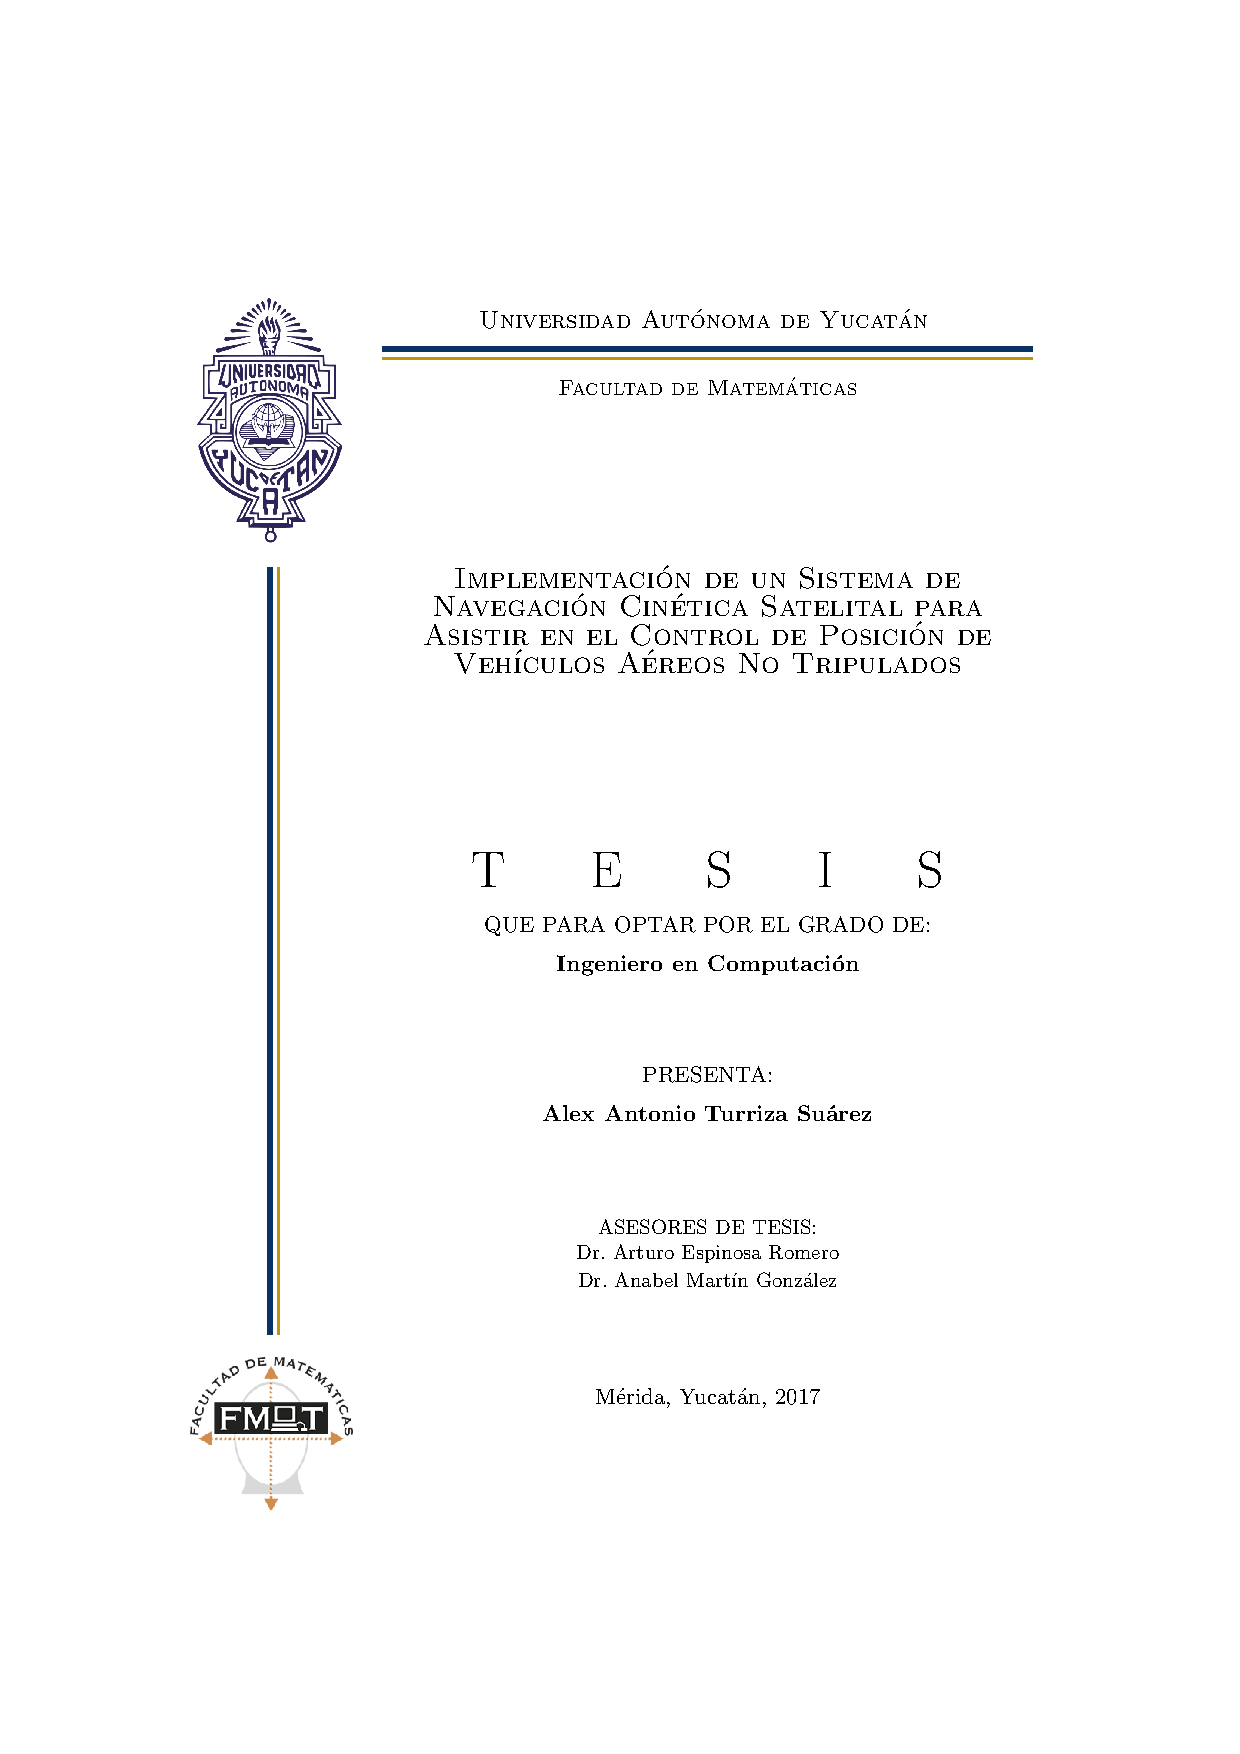
\includepdf[pages=-]{../PORTADA}
\afterpage{\blankpage}
%----------------------------------------------------------------------------------------
%	DECLARATION PAGE
%----------------------------------------------------------------------------------------

\begin{declaration}
\addchaptertocentry{\authorshipname} % Add the declaration to the table of contents
\noindent Yo, \authorname, declaro que este trabajo de tesis titulado, \enquote{\ttitle} y los resultados presentados son de mi autoría. Declaro que que:

\begin{itemize} 
\item Este trabajo fue realizado durante mi estancia como estudiante de la Facultad.
\item Ninguna parte de esta tesis ha sido previamente presentada para la obtención de un grado u otra promoción en esta Universidad u otra institución.
\item Todas las consultas a trabajos de otras personas han sido claramente atribuidos a sus respectivos autores.
\item Donde se hayan realizado citas textuales del trabajo de otras personas, la fuente siempre estará dada. Con la excepción de dichas citas, esta tesis es totalmente mía.
\end{itemize}
 
\noindent Firma:\\
\rule[0.5em]{25em}{0.5pt} % This prints a line for the signature
 
\noindent Fecha:\\
\rule[0.5em]{25em}{0.5pt} % This prints a line to write the date

\afterpage{\blankpage}

\end{declaration}

%----------------------------------------------------------------------------------------
%	QUOTATION PAGE
%----------------------------------------------------------------------------------------
\newpage
\vspace*{0.4\textheight}

\noindent\enquote{\itshape Si quieres hacer una tarta de manzana desde cero, primero debes inventar un universo.}\bigbreak

\hfill Carl Sagan


\afterpage{\blankpage}
%----------------------------------------------------------------------------------------
%	ABSTRACT PAGE
%----------------------------------------------------------------------------------------

\begin{abstract}
\addchaptertocentry{\abstractname} % Add the abstract to the table of contents
El conocimiento del entorno que nos rodea ha sido tema de interés humano desde antaño, así como la interacción con éste en el día a día, para poder investigar diferentes maneras en cómo se pueden aprovechar los recursos disponibles. Unas herramientas para describir el medio geográfico son los mapas realizados a mano; sin embargo, en lugar de ser una herramienta de exactitud, son sólo una referencia del entorno, dado el gran error derivado de la inexactitud humana en las mediciones.

En el presente trabajo se propone la implementación de un sistema de navegación cinética satelital para vehículos aéreos no tripulados (UAV, por sus siglas en inglés), que sea capaz de proporcionar una precisión muy alta (medible en centímetros) de forma que represente un apoyo en la planeación de rutas y ejecuciones de determinadas tareas cada cierta distancia que permitan la creación de mapas de imágenes aéreas más precisos.

Para alcanzar el objetivo, se trabajará con ayuda de software de procesamiento para RTK, que servirá de apoyo al momento de alcanzar la precisión deseada, además de dispositivos de hardware tales como un par de receptores GPS comunicados de forma inalámbrica, indispensables para implementar una corrección de tipo diferencial.
\end{abstract}

\afterpage{\blankpage}

%----------------------------------------------------------------------------------------
%	ACKNOWLEDGEMENTS
%----------------------------------------------------------------------------------------

\begin{acknowledgements}
\addchaptertocentry{\acknowledgementname} % Add the acknowledgements to the table of contents
\textit{A mis padres} \textbf{Antonio y Lucy}, aquellos que sin importar las circunstancias me apoyaron de principio a fin en esta odisea de estudiar un nivel superior en una ciudad aparte de donde soy originario. A mi \textit{hermana menor} \textbf{Haydeé Krystel}, quien estaba ahí para poder platicar conmigo y animarme en aquellos momentos donde lo necesité en estos años. Mención especial a mis abuelitos y mis tíos, tías, primos y primas, que siempre me apoyaron y me enseñaron muchas cosas y utilidades de sus vidas. \\

\textit{A mis asesores de tesis}, \textbf{Dr. Arturo Espinosa Romero y Dr. Anabel Martín González}, por la innumerable cantidad de conocimientos transmitidos que me serán de utilidad en el resto de la vida, en futuros retos, y por su infinita paciencia ante mis dudas y adversidades especialmente durante la realización de este trabajo. Mención especial a todos mis profesores, no sólo de la universidad. \\

\textit{A mi grupo de cercanos amigos:} Ernesto[\textbf{Nestor9224}], Kevin[\textbf{Kevan357}], Rafa[\textbf{RFer93}], Oscar[\textbf{MadOsc}], George[\textbf{El Tío}], Beto[\textbf{Ax Owl xA}] por estos años reuniéndonos para despejar la mente con los videojuegos como excusa. Junto conmigo, Alex[\textbf{AlexRT07}] somos \textit{los inútiles}, o mejor dicho, [TeamGG]\textbf{Los Gansos Galácticos}. \\

\textit{A mis compañeros de la carrera} por compartir cada momento no sólo en la estancia en la facultad y hacer de esta experiencia universitaria algo más agradable. \\

\textbf{\textit{\Large Muchas gracias a todos.}}

\end{acknowledgements} 
%----------------------------------------------------------------------------------------
%	LIST OF CONTENTS/FIGURES/TABLES PAGES
%----------------------------------------------------------------------------------------

\tableofcontents % Prints the main table of contents

\listoffigures % Prints the list of figures

\listoftables % Prints the list of tables

%----------------------------------------------------------------------------------------
%	ABBREVIATIONS
%----------------------------------------------------------------------------------------

\begin{abbreviations}{ll} % Include a list of abbreviations (a table of two columns)

\textbf{GPS} & \textbf{G}lobal \textbf{P}ositioning \textbf{S}ystem\\
\textbf{RTK} & \textbf{R}eal-\textbf{T}ime \textbf{K}inematics\\

\end{abbreviations}

%----------------------------------------------------------------------------------------
%	PHYSICAL CONSTANTS/OTHER DEFINITIONS
%----------------------------------------------------------------------------------------

\begin{constants}{lr@{${}={}$}l} % The list of physical constants is a three column table

% The \SI{}{} command is provided by the siunitx package, see its documentation for instructions on how to use it

Rotación de la Tierra & $r_{Earth}$ & \SI{460}{\meter\per\second} \\
%Constant Name & $Symbol$ & $Constant Value$ with units\\

\end{constants}

%----------------------------------------------------------------------------------------
%	SYMBOLS
%----------------------------------------------------------------------------------------

\begin{symbols}{lll} % Include a list of Symbols (a three column table)

$a$ & distance & \si{\meter} \\
$P$ & power & \si{\watt} (\si{\joule\per\second}) \\
%Symbol & Name & Unit \\

\addlinespace % Gap to separate the Roman symbols from the Greek

$\omega$ & angular frequency & \si{\radian} \\

\end{symbols}

%----------------------------------------------------------------------------------------
%	DEDICATION
%----------------------------------------------------------------------------------------

\dedicatory{Dedicado a todas aquellas personas que hacen especial mi vida...} 

%----------------------------------------------------------------------------------------
%	THESIS CONTENT - CHAPTERS
%----------------------------------------------------------------------------------------

\mainmatter % Begin numeric (1,2,3...) page numbering

\pagestyle{thesis} % Return the page headers back to the "thesis" style

% Include the chapters of the thesis as separate files from the Chapters folder
% Uncomment the lines as you write the chapters

% Chapter 1

\chapter{Introducción} % Main chapter title

\label{Chap:Intro} % For referencing the chapter elsewhere, use \ref{Intr} 

%----------------------------------------------------------------------------------------

% Define some commands to keep the formatting separted from the content 
\newcommand{\keyword}[1]{\textbf{#1}}
\newcommand{\tabhead}[1]{\textbf{#1}}
\newcommand{\code}[1]{\texttt{#1}}
\newcommand{\file}[1]{\texttt{\bfseries#1}}
\newcommand{\option}[1]{\texttt{\itshape#1}}

%----------------------------------------------------------------------------------------

\section{Preliminares}
En este documento de tesis se presenta la implementación de un sistema de navegación RTK (Real-Time Kinematics\footnotemark) con el apoyo de un software dedicado a navegación en una computadora portátil de bajo costo, basándose en el trabajo de \cite{takasu2009development}.

\footnotetext{Sistema de Navegación en Tiempo Real por sus siglas en inglés.}

\section{Importancia del tema}
La humanidad ha estado interesada en obtener información acerca del contexto en el que interactúa para poder utilizarlo a su favor. \\

A través del tiempo, se ha aumentado la certeza de los datos contenidos, por ejemplo, en un mapa, debido al aumento de la precisión de las herramientas de medición utilizadas. Un ejemplo de dichas herramientas son las computadoras, sensores y actuadores, así como de algoritmos que permiten filtrar errores aleatorios. \\

Mediante el uso de un sistema de navegación en tiempo real (RTK), se tiene como finalidad obtener la información de navegación de un vehículo de forma que este sistema pueda aportar datos confiables medibles en pocos decímetros para apoyar en el control de posicionamiento del mismo.

\section{Planteamiento del Problema}
A pesar del avance de la tecnología en las herramientas de medición, aún persisten algunos errores en la precisión, que de forma práctica, afectan al implementar sistemas basados en ellos. \\

\begin{figure}[H]
\centering
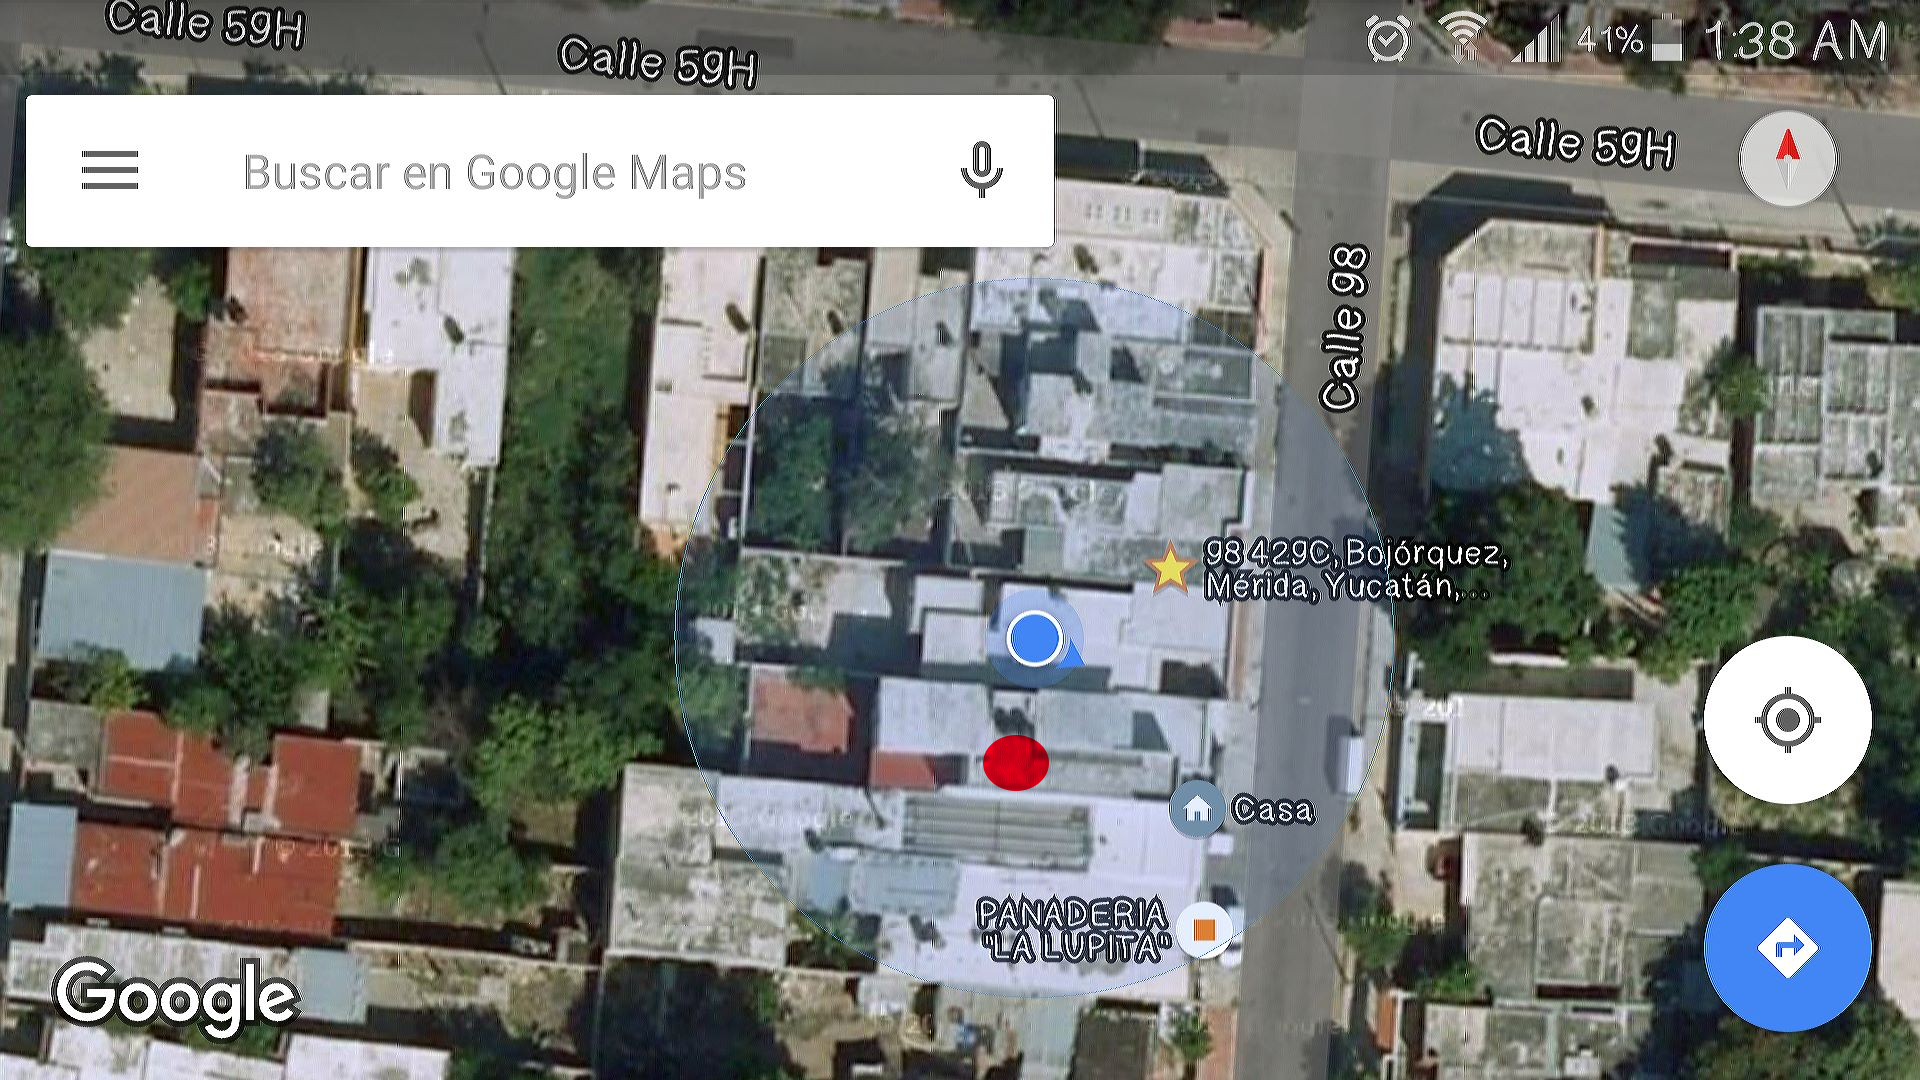
\includegraphics[scale=0.2]{Figures/Pred}
\caption[Posición de celular en mapa.]{Posición aproximada de la ubicación de un celular en un mapa de Google Maps.}
\label{fig:Prec}
\end{figure}

En una planeación de ruta de un sistema de navegación autónomo, decir que se conoce la posición de un objeto con un error de $n$ metros a la redonda de un punto dado, hace posible que dicho objeto se encuentre en cualquier lugar entre dicho punto y $n$ metros a la redonda, haciéndolo de consideración. Por ejemplo, al lanzar en la línea de costa a un helicóptero de juguete y volar un cierto tiempo, si se le pide que mediante GPS retorne al punto de inicio, se podría terminar con el juguete acuatizando varios metros dentro del mar. Como se puede observar en la figura~\ref{fig:Prec}, todo el círculo azul denota la posición aproximada de un dispositivo celular con GPS, y en donde la pequeña elipse roja muestra la posición real en dicho mapa. La circunferencia del círculo azul abarca prácticamente la mitad de una manzana, haciendo notorio un problema de impracticidad al intentar implementar un sistema de posicionamiento de, por ejemplo, un automóvil autónomo.

\section{Trabajos previos}
En la tesis de \cite{de2011diseno}, se usa un sistema GPS (Global Positioning System\footnotemark) para apoyar en la logística de distribución de farmacéuticos, como control de rutas, tiempos y seguridad, mencionando ante todo la capacidad de poder obtener los datos de localización y tiempo, además de la velocidad de desplazamiento de un vehículo. Sin embargo, de acuerdo al artículo de \cite{mendoza2004recomendaciones}, donde se propone una actualización del ancho de carriles carreteros a una amplitud adecuada máxima de 3.6 m, dado que un GPS mide su incertidumbre en una escala de metros, podría indicar que el vehículo se encuentra fuera de la cinta asfáltica o circulando en una vía contraria. Por tanto, se hace importante que un sistema tenga un menor grado de incertidumbre al ofrecido de forma estándar con GPS, como el Real-Time Kinematics, medido en pocos decímetros de error. \\

\footnotetext{Sistema de Posicionamiento Global, por sus siglas en inglés.}

También, la tesis escrita por \cite{ronnback2000developement}, menciona la implementación de un sistema de navegación inercial INS/GPS para un VANT (Vehículo Aéreo No Tripulado\footnotemark). Entre los datos a destacar, la posición de este sistema es estimada con un error de 2 m con un 95\% de confianza, además de otros datos para asistir al vuelo como velocidad y su altitud. Una incertidumbre de 2 m hace inviable que un drone (vehículo aéreo no tripulado) pudiese mantenerse cuando se le requiere que esté estático, por ejemplo, en fotografía aérea.\\

\footnotetext{Unmanned Aerial Vehicle, por sus siglas en inglés.}

Revisando el artículo de \cite{maldonado2010controlador}, los autores afirman que las coordenadas recibidas de un dispositivo GPS solamente son usadas como aproximación a la posición del vehículo, y nunca como un dato sólido que sirviese al computar datos, dada la exactitud mínima de 10 metros. Sin embargo, mencionan limitantes tales como el peso total de la carga del UAV y el consumo de energía causado por la integración de todos los demás sensores, de donde el GPS aporta entonces una cantidad mínima de información y utilidad en general. Sería ideal que el sistema de posicionamiento aportara información más precisa y que aporte a las observaciones realizadas con el vehículo de forma general.\\


\subsection{Propuesta}
Dado que en los trabajos previos se presentan algunos inconvenientes con la presición del sistema de navegación inercial de los dispositivos debido a la naturaleza del sensor GPS común utilizado, se propone la realización de un sistema de navegación que utilice una aplicación de cómputo denominada RTKLIB, que nominalmente reduce el error a una escala medible en centímetros a partir de dos señales de GPS, en un sistema portátil de arquitectura ARM (Advanced RISC Machine), ampliando las posibilidades de aprovechamiento de los datos.

\section{Hipótesis}
Mediante corrección diferencial de tipo Real-Time Kinematics, se puede reducir la incertidumbre de un equipo GPS a niveles de escasos decímetros.

\section{Objetivo}
\subsection{General}
El objetivo general de este trabajo es el diseño y la implementación de un sistema de navegación capaz de conocer su ubicación en un entorno geográfico con una alta precisión para apoyar en proyectos que requieran de dicha información, utilizando dispositivos pequeños y portátiles.

\subsection{Objetivos específicos}
\begin{itemize}
	\item Configurar los GPS en dos estaciones: una móvil y una base.
    \item Configurar la transferencia de datos entre estaciones en UHF (Ultra-High Frequency\footnotemark).
    \footnotetext{Ultra-Alta Frecuencia, por sus siglas en inglés.}
    \item Acondicionamiento de una microcomputadora BeagleBone con sus respectivos periféricos de apoyo.
    \item Programación de una biblioteca que controle los periféricos a través de la microcomputadora.
    \item Integración de módulos.
	\item Evaluación de los datos obtenidos.   
\end{itemize}

\section{Publicaciones}

Los avances de este proyecto fueron publicados en las memorias en extenso del Encuentro Universitario de Sistemas Computacionales - EUSICS 2016, editado por \citet{eusics}.

\section{Descripción del documento}

El presente trabajo se divide en las siguientes secciones: 

\begin{itemize}
\item \textbf{Introducción:} Se describen tanto la importancia del tema, los problemas a resolver, estado del arte, y una lista de objetivos a seguir durante el desarrollo del tema.\\
\item \textbf{Marco Teórico:} En este apartado se sientan las bases de funcionamiento de los dispositivos a utilizar, así como información útil acerca de los mismos. Se da una descripción general tanto del hardware como del software utilizado.\\
\item \textbf{Diseño del Hardware y Software:} En esta sección se enlistan diversos recursos implementados en el trabajo, tanto de software como de hardware. Se da una descripción de cada uno y el aporte que tienen a la estructura final durante el funcionamiento.\\
\item \textbf{Diseño del Experimento:} Se describen las condiciones a las que será sometido el prototipo para indicar un adecuado funcionamiento de acuerdo a los objetivos listados en la introducción.\\
\item \textbf{Análisis de Resultados:} Se realiza una evaluación de los resultados obtenidos durante la ejecución de la rutina experimental. Se enfatizan diferencias de los distintos modos de funcionamiento y su impacto en el rendimiento del sistema.\\
\item \textbf{Conclusiones:} En forma de síntesis, se da un resumen de los resultados obtenidos de acuerdo al modo de funcionamiento, las observaciones  y el rendimiento en general del sistema.\\
\end{itemize}

Además, al final se añade una sección de anexos en donde se adjuntan guías de configuración o programación de distintos dispositivos de hardware o de software necesarios para la reproducción del proyecto.\\

%En el capítulo~\ref{Chap:Marco}, se expone la teoría que se encuentra detrás de la metodología implementada en el proyecto de tesis, partiendo desde la definición de un sistema GPS, pasando por su modo de funcionamiento y las principales causas de error en sus mediciones. También, se presenta una breve descripción del funcionamiento de una comunicación inalámbrica, del software y del hardware utilizado.
% Chapter 2

\chapter{Marco Teórico} % Main chapter title

\label{Chap:Marco} % For referencing the chapter elsewhere, use \ref{Chapter2} 

%----------------------------------------------------------------------------------------

% Define some commands to keep the formatting separated from the content 
%\newcommand{\keyword}[1]{\textbf{#1}}
%\newcommand{\tabhead}[1]{\textbf{#1}}
%\newcommand{\code}[1]{\texttt{#1}}
%\newcommand{\file}[1]{\texttt{\bfseries#1}}
%\newcommand{\option}[1]{\texttt{\itshape#1}}

%----------------------------------------------------------------------------------------

\section{Introducción}

En esta sección se presenta la teoría de varios elementos clave en el prototipo a utilizar. Partiendo desde la definición de GPS, pasando por una breve historia, su fundamento matemático y las causas de error en las mediciones, hasta el software utilizado y los dispositivos específicos utilizados en este trabajo, se presentan datos de funcionamiento y su relación con el proyecto.

\section{El Sistema de Posicionamiento Global - GPS}

\begin{figure}[ht]
\centering
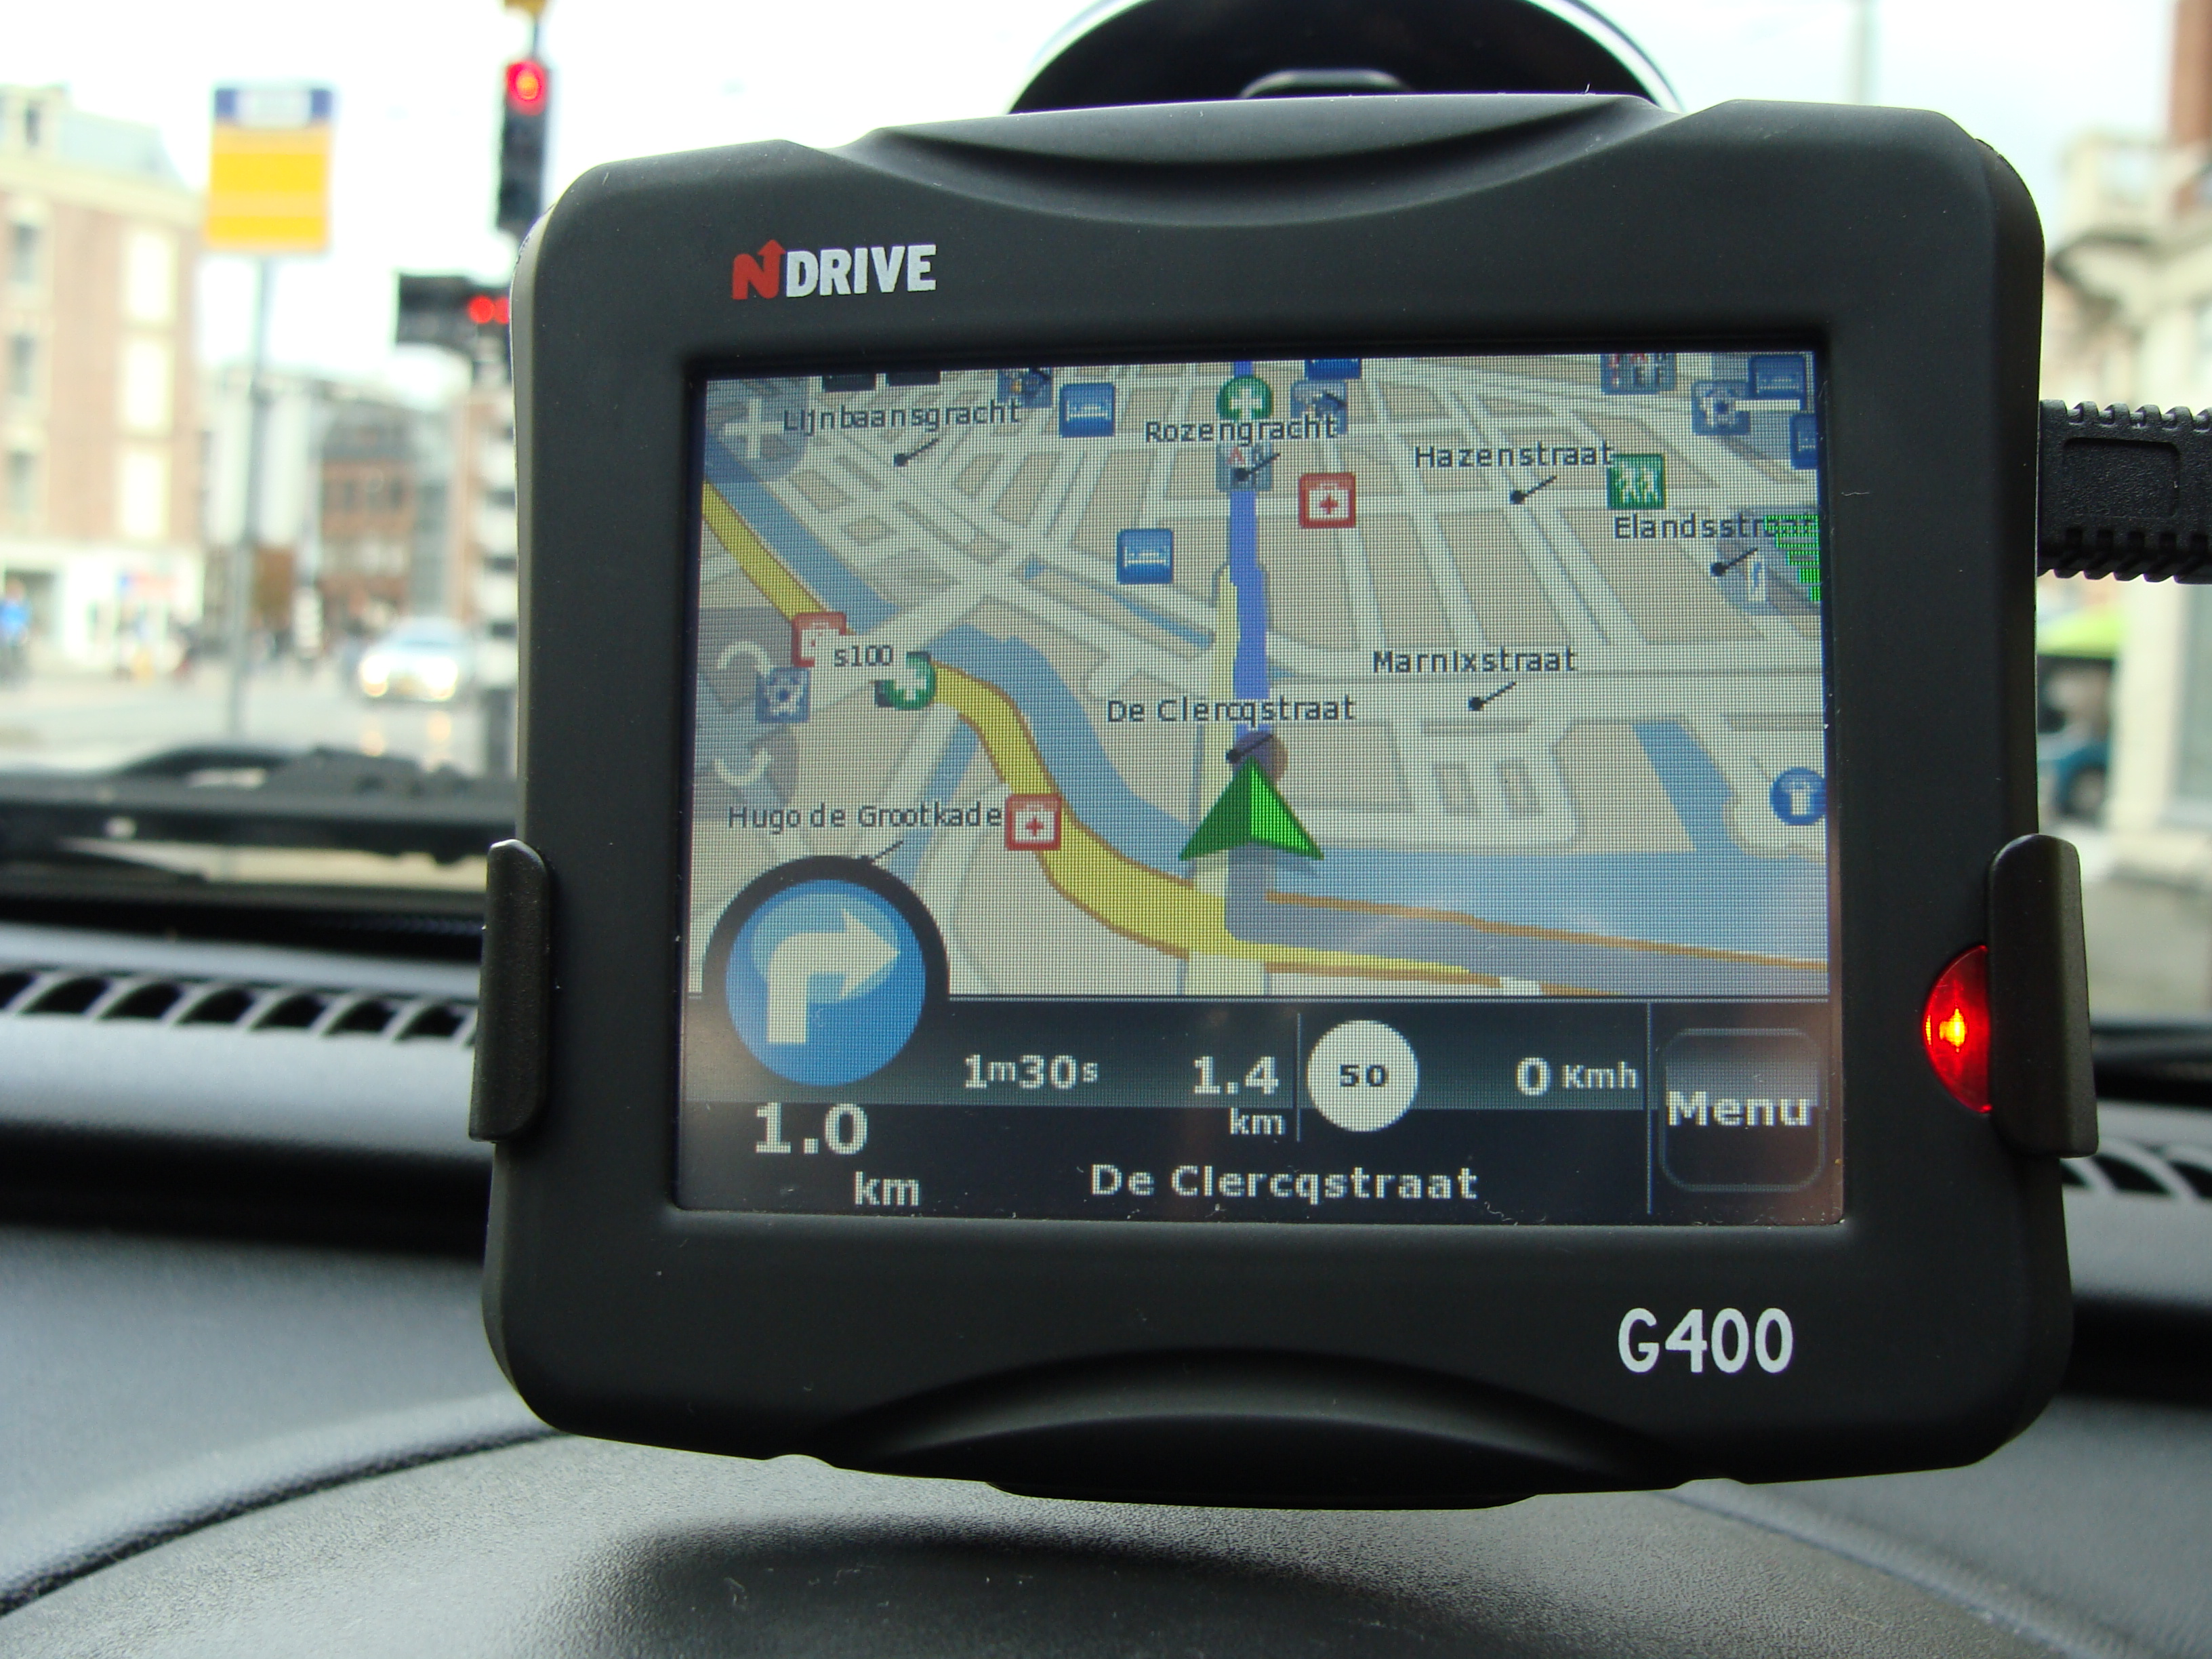
\includegraphics[scale=0.12]{Figures/GPS}
\caption[Sistema de Posicionamiento Global.]{Sistema de Posicionamiento Global.\footnotemark}
\label{fig:GPS}
\end{figure}

\footnotetext{Imagen tomada de: \href{https://upload.wikimedia.org/wikipedia/commons/thumb/9/9f/NDrive_GPS.jpg/1280px-NDrive_GPS.jpg}{https://upload.wikimedia.org/}}

GPS fue iniciado en 1973 para su uso con fines militares por los Estados Unidos de Norteamérica. Su objetivo principal es la determinación de las coordenadas espaciales bajo una referencia mundial. Para dichos propósitos, se necesita una recepción de señales de un mínimo de cuatro satélites, cuyas coordenadas son plenamente conocidas \citep{huerta2005gps}.

\subsection{Historia}

\subsubsection{Antecedentes}
Antes de que GPS funcionara mediante satélites, ya estaban implementados varios sistemas de localización radio-terrestres. Uno de ellos era conocido como LORAN (\textit{Long Range Navigation}, Navegación de largo alcance por sus siglas en inglés). Se fundamentaba por el envío de una señal desde distintos emisores. Al percibir señal de tres distintos emisores, podía determinar su posición. \\

Fue tras el lanzamiento del Sputnik\footnotemark, que investigadores norteamericanos descubrieron que era posible la determinación de la posición gracias a la deformación de una señal por efecto Doppler. Así, si era posible conocer la posición del satélite conociendo la posición del observador en la Tierra, a la inversa, sería posible conocer la posición de un observador conociendo la posición del satélite.

\footnotetext{Satélite ruso, el primero de la historia.}

\subsubsection{Con satélites en órbita}
El primer sistema que utilizaba la triangulación mediante satélites fue \textit{TRANSIT} en 1960, entrando en operaciones hasta 1965. Constaba de seis satélites en seis planos, contando con cobertura mundial. \\

Requería que el observador realizara un seguimiento de 15 minutos a la constelación satelital, pudiendo acceder a ellos cada hora y media. Su error de precisión rondaba los 250 metros.\\

En 1973 se propuso el \textit{DNSS} (Defense Navigation Satellite System, Sistema de Navegación Satelital de Defensa por sus siglas en inglés), cambiando de nombre a \textit{NAVSTAR} (Navigation System Time and Ranging, Sistema de Navegación por Tiempo y Distancia, por sus siglas en inglés), después a \textit{NAVSTAR-GPS} y finalmente a \textit{GPS} \citep{termal2014prototipo}.

\subsection{La constelación NAVSTAR}

\begin{figure}[H]
\centering
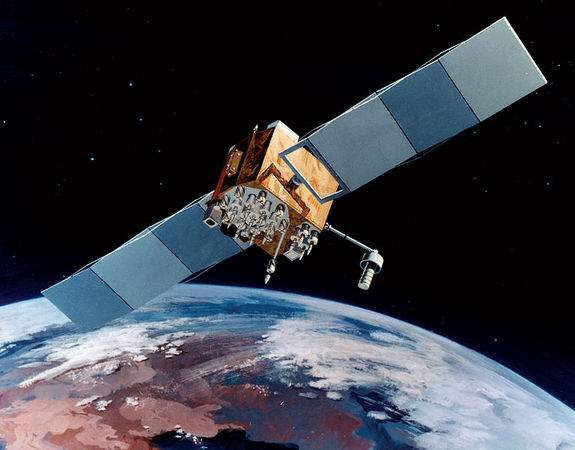
\includegraphics[scale=0.95]{Figures/Navstar}
\caption[Satélite de la constelación NAVSTAR.]{Satélite de la constelación NAVSTAR\footnotemark.}
\label{fig:NAV}
\end{figure}

\footnotetext{Imagen tomada de: \href{https://upload.wikimedia.org/wikipedia/commons/thumb/f/f4/Navstar-2F.jpg/613px-Navstar-2F.jpg}{https://upload.wikimedia.org/}}

La constelación \textit{NAVSTAR} está conformada por los satélites que se utilizan para triangular la posición. Se propuso que fueran 24 satélites situados en seis planos de cuatro satélites cada uno, con cobertura en toda la Tierra. \\

La constelación ha sido lanzada en conjuntos llamados \textit{Blocks} (bloques en inglés), distribuidos de la siguiente manera, de acuerdo al artículo de \cite{termal2014prototipo}.

\begin{itemize}
	\item Block I (1978 - 1985): 11 satélites lanzados, \textcolor{blue}{10 puestos en órbita con éxito}.
	\item Block II (1989 - 1990): \textcolor{blue}{9 satélites puestos en órbita con éxito}.
	\item Block IIA (1990 - 1997): \textcolor{blue}{19 satélites lanzados con éxito}.
	\item Block IIR (1997 - 2004): 11 satélites lanzados, \textcolor{blue}{12 satélites lanzados con éxito}.
	\item Block IIR-M (2005 - 2009): \textcolor{blue}{8 satélites lanzados con éxito}.
	\item Block IIF (2010): \textcolor{blue}{1 satélite lanzado con éxito}.
\end{itemize}

\subsection{Estructura}

GPS está conformado por tres segmentos:

\begin{itemize}
	\item Segmento espacial: los satélites.
	\item Segmento de control: estaciones terrestres.
	\item Segmento de usuario: los receptores.
\end{itemize}
	
\subsubsection{Segmento espacial}

Se conoce como segmento espacial al sistema de satélites que orbitan al planeta Tierra, emitiendo señales que permiten al receptor calcular su posición en el marco de referencia terrestre. \\

\begin{figure}[H]
\centering
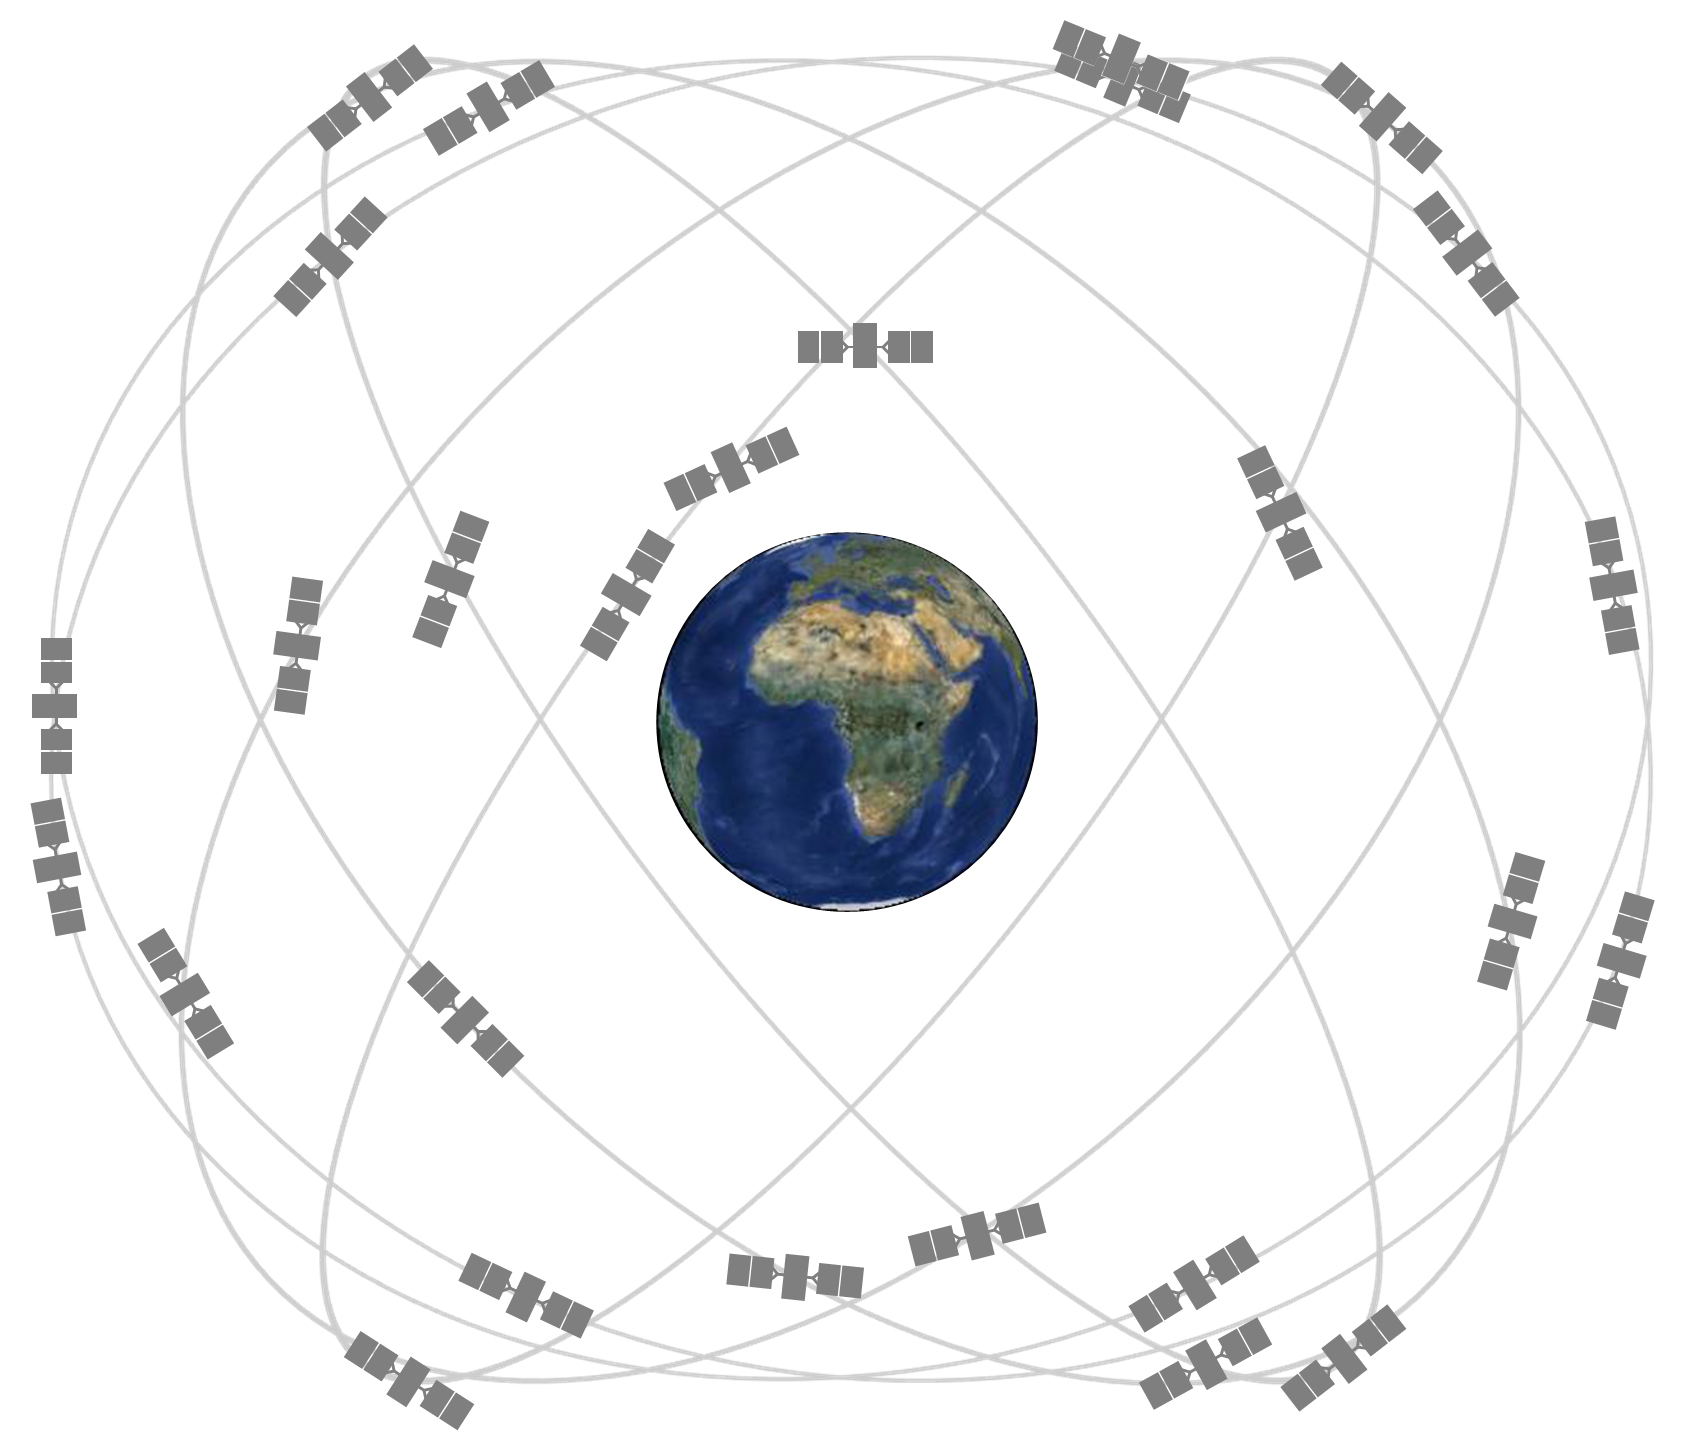
\includegraphics[scale=0.2]{Figures/constel}
\caption[Segmento espacial.]{Segmento espacial.\footnotemark.}
\label{fig:segEs}
\end{figure}

\footnotetext{Imagen tomada de \href{http://www.gps.gov/multimedia/images/constellation.jpg}{http://www.gps.gov/}}

Se reparten en seis órbitas sincronizadas y se desplazan a una altitud de 20'000 Km. Cada uno de ellos dan una vuelta a la Tierra en 12 horas. \\

Como ejemplifica la figura~\ref{fig:segEs}, los planos orbitales están equitativamente separadas de forma que se garantice virtualmente que desde cualquier punto del planeta, un mínimo de 4 satélites sean visibles, siendo éste el número mínimo para un funcionamiento adecuado. Cada órbita contiene 4 satélites, haciendo un total de 24 equipos rodeando al planeta. Hasta la fecha, existen 3 satélites denominados extra. Estos equipos están hechos tanto para mejorar la cobertura de los 24 originales, o bien, sustituir a alguno en caso de presentarse una falla o termine su ciclo de vida \citep{gps_gov}.\\

Los satélites son ajustados mediante mensajes NAV enviados desde el segmento de control.

\subsubsection{Segmento de control}

Conjunto de sistemas instalados en la Tierra que permiten el funcionamiento óptimo del segmento espacial.\\

Conformada por 12 estaciones, de las cuales la principal \textit{MCS} (Master Control Station\footnotemark) se encuentra en Colorado, en la Base Schriever de la Fuerza Aérea.\\

\footnotetext{Estación de Control Principal por sus siglas en inglés.}

Tras el envío de nueva información, cada satélite sincroniza su reloj atómico y ajusta las efemérides de su órbita. El cálculo de esta última es a través de un filtro de Kalman, permitiendo una estimación precisa a pesar de múltiples factores externos.

\subsubsection{Segmento de usuario}

Conformado por equipos receptores diseñados para recibir, decodificar y procesar las señales de los satélites. Los parámetros para controlar la calidad de los receptores utilizados son los siguientes, de acuerdo a \citep{termal2014prototipo}:

\begin{itemize}
	\item La antena debe estar bajo cielo abierto recibiendo la señal de los satélites con suficiente potencia.
	\item El reloj interno del receptor debe mantener la sincronización entre receptor y satélites.
	\item El número de canales debe habilitar al receptor para sintonizar un número suficiente de señales.
	\item El procesador debe tener una frecuencia tal que garantice un cálculo correcto de la posición a partir de las señales captadas.	
\end{itemize}

El segmento espacial y el segmento de usuario están conectadas por dos frecuencias inalámbricas: \textbf{L1} y \textbf{L2}. La primera es de 1575.42 MHz y la segunda de 1227.60 MHz \citep{farrell2008aided}.

\subsection{Dispositivos GPS}
Los dispositivos GPS son aparatos receptores que obtienen la información de los satélites y realizan un procesamiento del mismo para ubicarse en el marco de referencia terrestre. \\

Existen GPS de distintos tamaños y marcas. La diferencia entre estas consiste en la velocidad del procesador, las frecuencias de los mensajes de los satélites que puede captar, su rango de operación y su velocidad de muestreo y actualización, y si es capaz de aplicar algún tipo de correcciones al momento. Algunos equipos pueden otorgar la información de sus observaciones sin procesar.

\begin{table}[H]
\begin{center}
\caption{Características del GPS Navspark RAW.}
\begin{tabular}{|l|}
	\hline
	        \ \ \ \ \ \ \ \ \ \ \ \ \ \ \ \ \ \ \ \ \ \ \ \ \ \ \ \ \ \ \ \ \ \ \ \ \ \ \ \ \ \ \ \ \ \ \ \ \ \ \textbf{Navspark RAW GPS} \\
	\hline
	%\begin{figure}[H]%Example image
		\\  \ \ \ \ \ \ \ \ \ \ \ \ \ \ \ \ \ \ \ \ \ \ \ \ \ \ \ \ \ \ \ \ \ \ \ \ \ \ \ \ 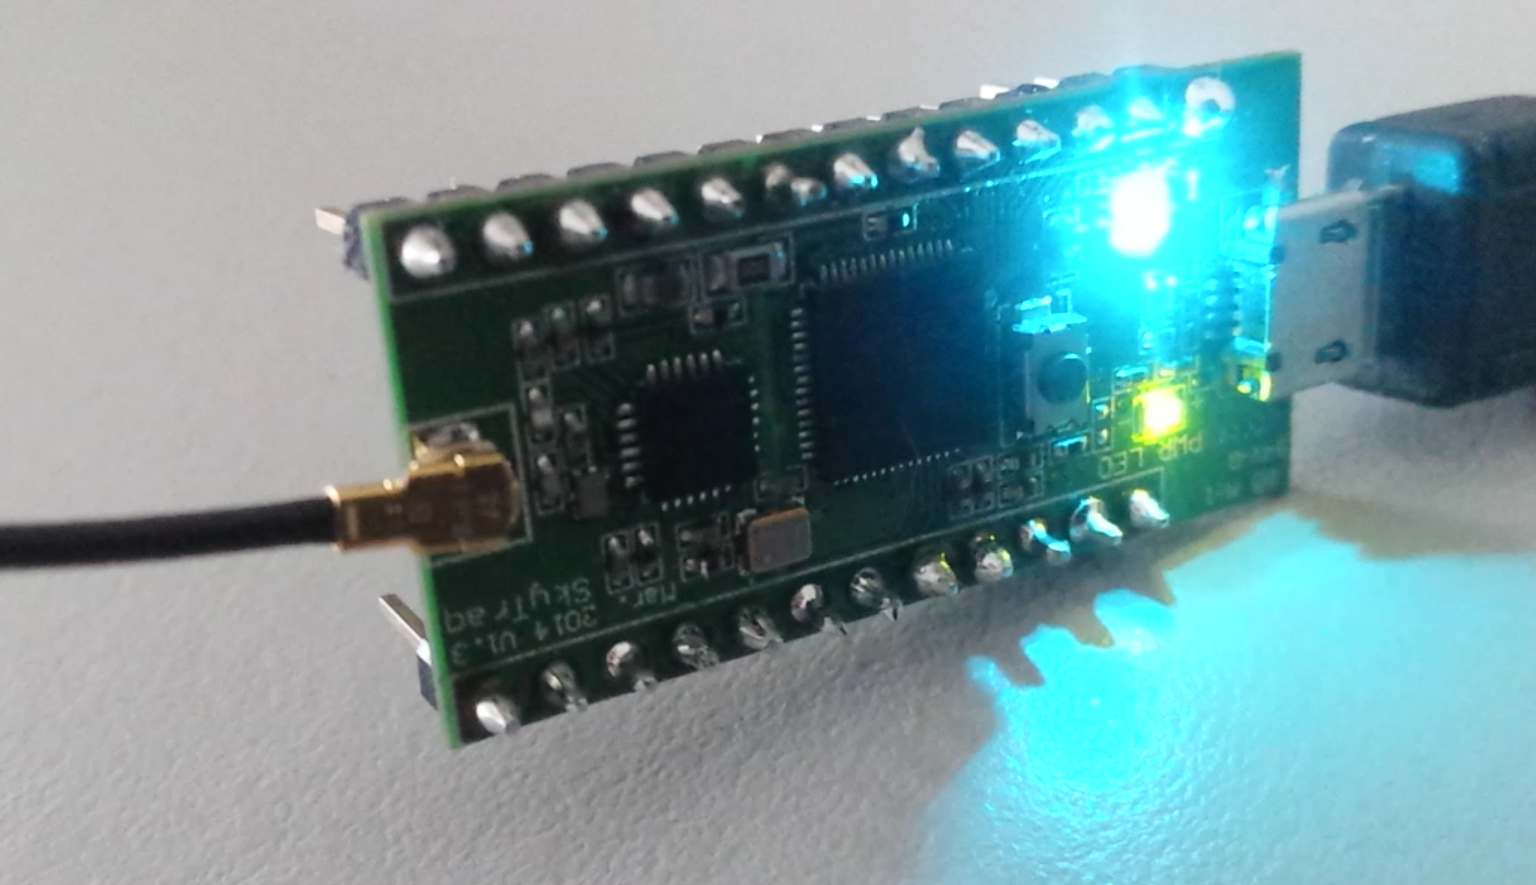
\includegraphics[width=0.37\linewidth]{Figures/NavGPS}
	%	\caption{GPS Navspark.}
		\label{fig:nsraw}\\
	%\end{figure} \\
	
	\textbf{Características:}\\
	%\begin{itemize}
		\tabitem Procesador: 100MHz 32bit LEON3 Sparc-V8 + IEEE-754 Compliant FPU.\\
		\tabitem 17 Digital I/O.\\
		\tabitem GPS con actualización de hasta 20 Hz.\\
		\tabitem Rango de operación: (h $<$ 18000 msnm) \& (v $<$ 515 m/s).\\
		\tabitem Precisión de hasta 2.5 metros.\\
		\tabitem Consumo: 15 ma @ 3.3V \citep{nsraw}.\\
	%\end{itemize} \\
	\hline
\end{tabular}
\end{center}
\end{table}

\begin{table}[H]
\begin{center}
\caption{Características del GPS Ublox C94 M8P.}
\begin{tabular}{|l|}
	\hline
	\ \ \ \ \ \ \ \ \ \ \ \ \ \ \ \ \ \ \ \ \ \ \ \ \ \ \ \ \ \ \ \ \ \ \ \ \ \ \ \ \ \ \ \ \ \ \ \textbf{Ublox C94 M8P GPS}\\
	\hline
	%\begin{figure}[H] % Example image
	      \ \ \ \ \ \ \ \ \ \ \ \ \ \ \ \ \ \ \ \ \ \ \ \ \ \ \ \ \ \ \ \ \ \ \ \ \ \ \ \ \ \ \ \ \ \ \ 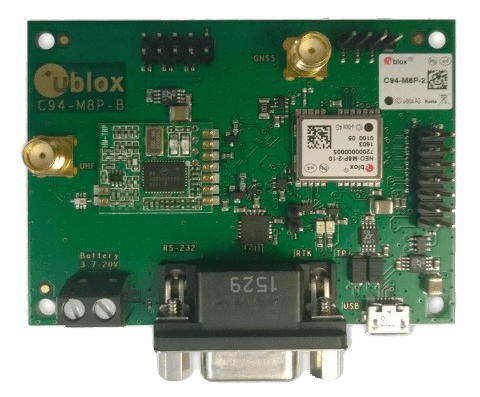
\includegraphics[width=0.25\linewidth]{Figures/ublox}\footnotemark
	%\caption{GPS Ublox. \footnotemark}
	\label{fig:ubx} \\
	%\end{figure} \\
	\textbf{Características: }\\

	%\begin{itemize}
		\tabitem 72 channel u-blox M8 engine GPS L1C/A, GLONASS L1OF, BeiDou B1.\\
		\tabitem GPS con actualizaciones de hasta 10 Hz.\\
		\tabitem Rango de operación: (h $<$ 50000 msnm) \& (v $<$ 500 m/s).\\
		\tabitem Precisión de hasta 2.5 metros.\\
		\tabitem Consumo: 23 ma @ 3.3V.\\
		\tabitem \textcolor{blue}{Incluye módulo de radiofrecuencia.} \citep{ubloxc94}.\\
	%\end{itemize} \\
	\hline
\end{tabular}
\end{center}
\end{table}

\footnotetext{Imagen alojada en www.u-blox.com}

\FloatBarrier

\newpage

\subsection{Principios de funcionamiento}

El objetivo de GPS como sistema de localización es el de calcular la posición de un punto cualquiera en un espacio de coordenadas (x,y,z) \citep{sonnenberg2013radar}, comenzando con el cálculo de las distancias del punto a un mínimo de tres satélites con localización conocida, dicha distancia se obtiene multiplicando el tiempo de propagación de la señal emitida por su velocidad de difusión.\\

Al error de distancias causado por el desfase temporal del reloj del receptor se le llama pseudodistancia \citep{pozo2000sistema}.


\subsection{Fundamento matemático}

En esta subsección se muestra una síntesis del libro de \cite{farrell2008aided}, del cálculo de la posición de los satélites.

A través de las frecuencias L1 y L2, el segmento espacial provee de cobertura a todo el planeta. \cite{farrell2008aided} menciona al \textbf{pseudorango} como aquel desfase en distancia causado por errores de medición causados por el reloj del dispositivo. El \textbf{pseudotiempo} lo define como el tiempo de tránsito del mensaje de los satélites a los aparatos GPS incluyendo el error. \\

El objetivo de un receptor GPS en cualquier parte de la Tierra es calcular su posición a través de la determinación de la posición de los satélites que enviaron sus datos de localización en un determinado momento.\\

Las variables importantes a utilizar están listados en el cuadro~\ref{Tab:TablaVariables}.

\begin{table}[!htb]
\begin{center}
\caption{Variables presentes en el cálculo de posiciones de satélites.}
\label{Tab:TablaVariables}
\begin{tabular}{|c|l|}
	\hline
	\multicolumn{2}{|c|}{\textbf{Variables}}\\
	\hline
	$t^{'}_r$ & El pseudotiempo en que el receptor toma una medición.\\
	\hline
	$t_{sv}$ & El pseudotiempo en el que un satélite emite la señal hacia los \\ & receptores.\\
	\hline
	$t^{'}_p$ & El pseudotiempo de propagación de la señal emitida por el satélite\\ & hasta llegar a la antena del receptor.\\
	\hline
	$\Delta t_{sv}$ & El sesgo del reloj satelital.\\
	\hline
	$t$ & El tiempo de GPS en el que el satélite emite la señal hacia los\\ & receptores.\\
	\hline 
	$b$ & El sesgo del reloj del receptor.\\
	\hline
	$t_r$ & El tiempo de GPS en el que el receptor toma una medición.\\
	\hline
	$t_p$ & El tiempo de propagación de la señal desde la antena del satélite\\ & hasta la antena del receptor.\\
	\hline
\end{tabular}
\end{center}
\end{table}

En la figura~\ref{fig:DiagMat} se puede observar a cada variable relacionada con el objeto que juega durante el proceso del cálculo de posición de los satélites. 

\begin{figure}[H]
\centering
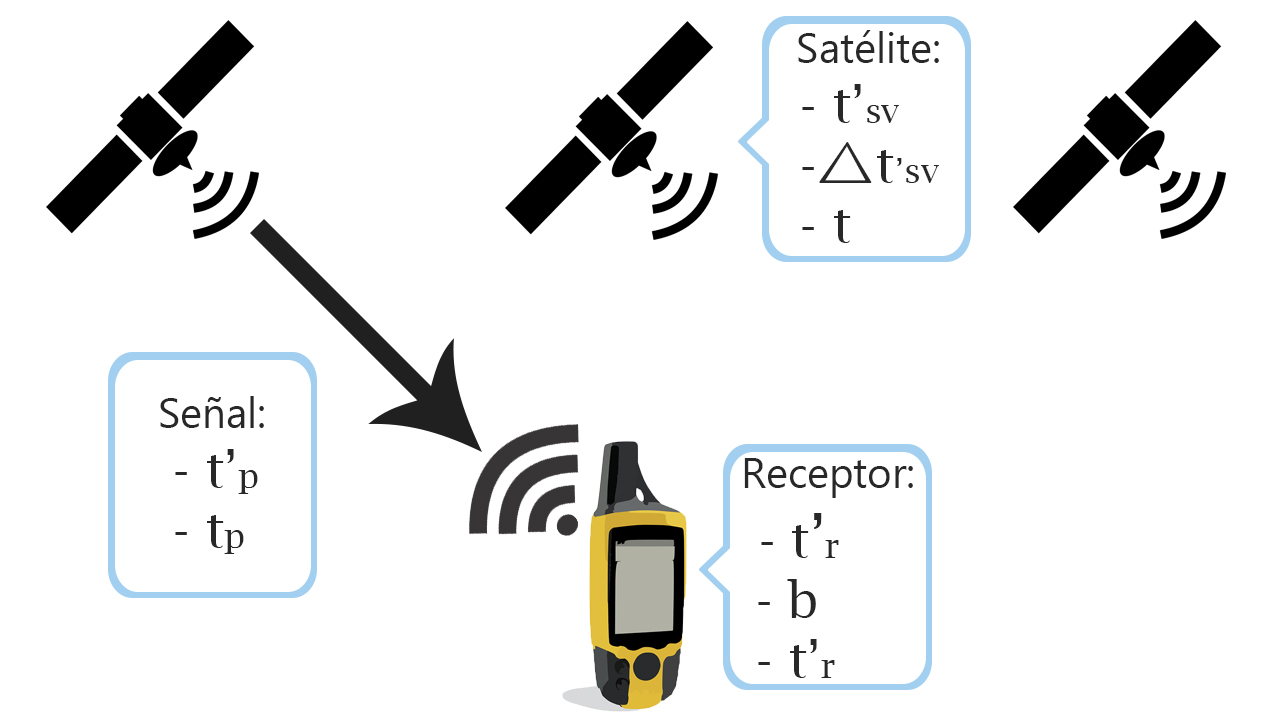
\includegraphics[scale=0.41]{Figures/DiagramaMat}
\caption[El rol que juega cada variable.]{El rol que juega cada variable.}
\label{fig:DiagMat}
\end{figure}

Las variables $t$ y $t_{sv}$ están dadas por: 

\begin{equation}
\label{Eq:tsv}
t_{sv} = t + \Delta t_{sv}
\end{equation}

Donde $t_{sv}$ es llamado el \textit{tiempo de canal}, porque el receptor mantiene un valor distinto para cada canal.\\

Las variables $t_r$ y $t^{'}_r$ están dadas por:

\begin{equation}
\label{Eq:t_r}
t^{'}_r = t_r + b
\end{equation}

Donde $t^{'}_r$ es el tiempo del receptor y es común para todos los canales. \\

El tiempo de propagación $t_p$ está dado por:

\begin{equation}
\label{Eq:t_p}
t_p = t_r - t
\end{equation}

Los valores típicos para $t_p$ rondan entre 60 ms y 90 ms. \\

Ahora, asumiendo que $b$ inicialmente es desconocida, el cálculo se resume como sigue:\\

\begin{itemize}
\item[1.] En el tiempo $t^{'}_r$, el receptor toma una muestra de todos los canales en los que encuentra señal.\\

\item[2.] En cada canal, el procesador del receptor calcula $t_{sv}$.\\

\item[3.] El procesador del receptor calcula el pseudotiempo de propagación y el pseudorango $\rho$ para cada canal.\\

\begin{equation}
\label{Eq:t'_p}
t^{'}_p = t^{'}_r - t_{sv}
\end{equation}

\begin{equation}
\label{Eq:rho}
\rho = ct^{'}_p
\end{equation}

Donde $c$ es la velocidad de la luz, cuyo valor se muestra en la lista de constantes físicas \ref{Chap:Const}.

\item[4.] Se calcula $\Delta t_{sv}$ utilizando la siguiente ecuación:

\begin{equation}
\label{Eq:Deltat_sv}
\Delta t_{sv}= a_{f0} + a_{f1}(t_{sv}-t_{oc}) + a_{f2}(t_{sv}-t_{oc})^2 + \Delta t_{r}
\end{equation}

Donde $t_{oc}$ y los coeficientes polinomiales son parte del mensaje de navegación proporcionado por los satélites.\\

El término $\Delta t_{r}$ es una corrección relativista:

\begin{equation}
\label{Eq:Deltat_r}
\Delta t_r = FeA^{1/2}sin(E_{k})
\end{equation}

$F$, $e$ y $A$ son constantes definidas en la lista de constantes físicas\ref{Chap:Const}.\\

$E_{k}$ es la ecuación de Kepler de la anomalía de la excentricidad, dada por:

\begin{equation}
\label{Eq:Kepler}
E_k = M_k + esin(E_k)
\end{equation}

Donde $M_k$ es la anomalía media en radianes, dada por: \\

$M_k = M_0 + t_k n$\\

Donde $t_k$ es el tiempo desde la época referenciada, dada por:\\

$t_k = t - t_{oe}$\\

Donde $t_{oe}$ es una constante dada en la observación satelital.\\

$M_0$ es una constante dada en la observación satelital\\

Y $n$ es la media de corrección de movimiento, en radianes por segundo (rps), dada por:\\

$n = n_0 + \Delta n$\\

Donde $n_0$ es la media de compensación de movimiento en rps, dada por:\\

$n_0 = \sqrt{\mu / A^{3}}$\\ 

Y $\Delta n$ es una constante dada por la observación.\\

\item[5.] Partiendo de que es posible calcular $\Delta t_{sv}$ con la ecuación~\ref{Eq:Deltat_sv}, se puede calcular $t$ utilizando la igualdad~\ref{Eq:tsv}, de la siguiente manera:

\begin{equation}
\label{t}
t = t_{sv} - \Delta t_{sv}
\end{equation}

Con $t$ calculada, es posible el cálculo de la posición de los satélites. Contando con dichas posiciones y las mediciones de pseudorangos, el receptor puede calcular su propia posición y el sesgo de reloj $b$.

\item[6.] El receptor ahora puede calcular $t_r$ y $t_p$.
\end{itemize}

\subsection{Causas de error}

Como en todo sistema de medición, es probable que un cálculo de una posición se vea afectado por cualquiera de las siguientes: 

\begin{itemize}
	\item Satélites.
	\item Atmósfera.
	\item Rutas múltiples.
	\item Receptor.
\end{itemize} 

\subsubsection{Error causado por el satélite}

\begin{figure}[H]
\centering
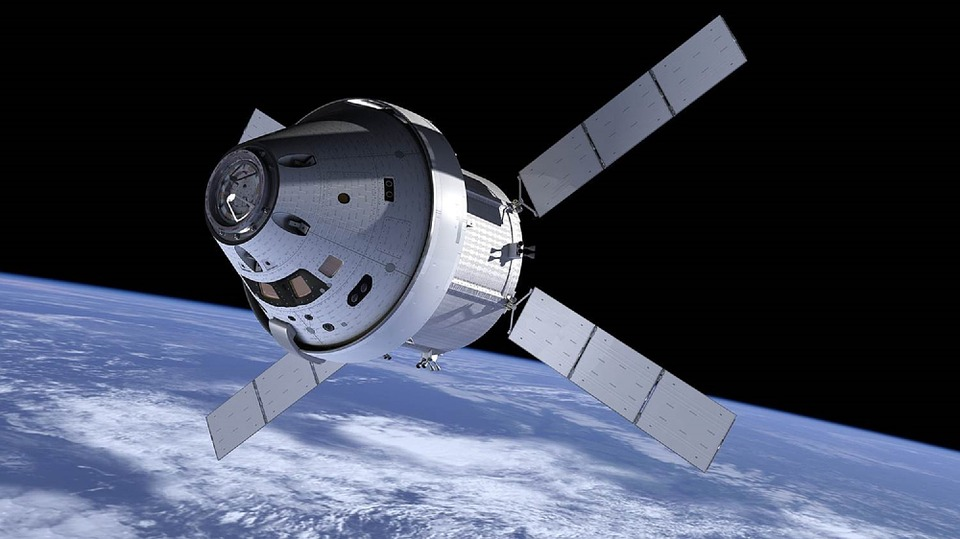
\includegraphics[scale=0.41]{Figures/Sat}
\caption[Error del reloj atómico satelital.]{Error del reloj atómico satelital\footnotemark.}
\label{fig:ErrSat}
\end{figure}

\footnotetext{Imagen tomada de: \href{https://pixabay.com/p-568635/?no_redirect}{https://pixabay.com/}}

Los satélites incorporan relojes atómicos de gran exactitud. Como el tiempo es crítico al momento de la triangulación de cualquier dispositivo, un error de apenas un nanosegundo equivale a un error en distancia de 30 cm. Los relojes atómicos acumulan un error de esta magnitud cada tres años. \\

También, al error en la posición de los satélites sobre sus órbitas se le atribuye un error de 2.1 metros.

\subsubsection{Error causado por la atmósfera}

\begin{figure}[H]
\centering
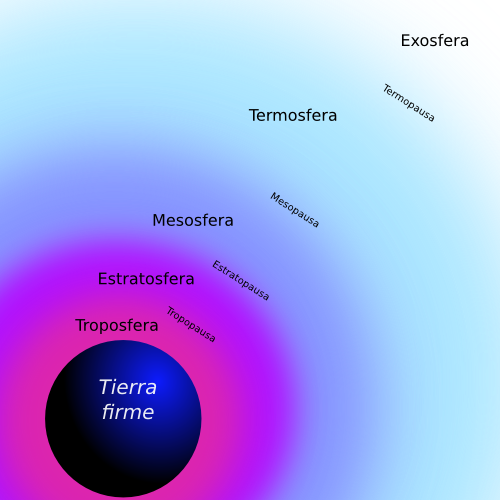
\includegraphics[scale=0.9]{Figures/CapasAtm}
\caption[Error por capas de la Atmósfera.]{Error por capas de la Atmósfera\footnotemark.}
\label{fig:ErrAtm}
\end{figure}

\footnotetext{Imagen tomada de: \href{https://upload.wikimedia.org/wikipedia/commons/0/03/Atmosferaterra.png}{https://upload.wikimedia.org/}}

Las señales de radio que comunican a los satélites y los receptores deben atravesar a la atmósfera a través de considerables kilómetros. El sólo hecho de atravesar partículas cargadas en la ionósfera\footnotemark y entrar en contacto con el vapor de agua de la tropósfera causa variaciones de velocidad en la transmisión. \\

El error en distancia atribuible a esta etapa es de 4 metros. 

\footnotetext{El error obtenido en la ionósfera puede eliminarse utilizando receptores de frecuencia doble L1 y L2.}

\subsubsection{Error causado por rutas múltiples}

\begin{figure}[H]
\centering
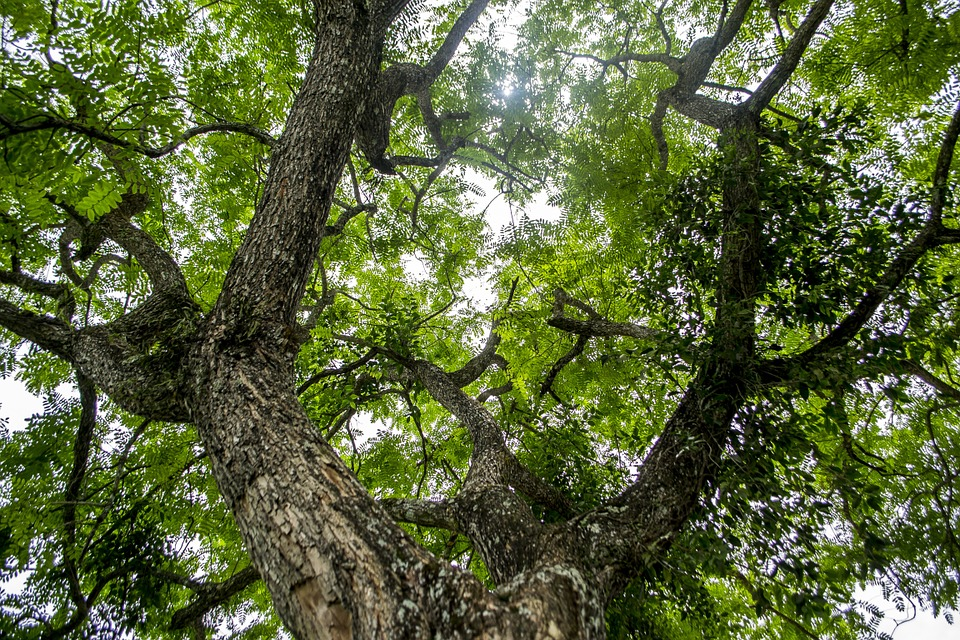
\includegraphics[scale=0.4]{Figures/RutasMult2}
\caption[Error por rutas múltiples.]{Error por rutas múltiples\footnotemark.}
\label{fig:ErrRMul}
\end{figure}

\footnotetext{Imagen tomada de: \href{https://pixabay.com/p-579199/?no_redirect}{https://pixabay.com/}}

 El sistema está diseñado para funcionar idealmente a cielo abierto. Sin embargo, en condiciones normales, esto no puede ser del todo reproducible, ya sea por el uso en áreas forestales o áreas urbanas. \\
 
Normalmente, la señal directa llega primero al receptor, y después, arriban las que proceden de las rutas múltiples. Esta diferencia de tiempo ocasiona otro error de medición. \\

Este mismo efecto era visible en las señales análogas de televisión, en las imágenes dobles. \\

Las nuevas antenas exteriores pueden filtrar este efecto.

\subsubsection{Error causado por el receptor}

\begin{figure}[H]
\centering
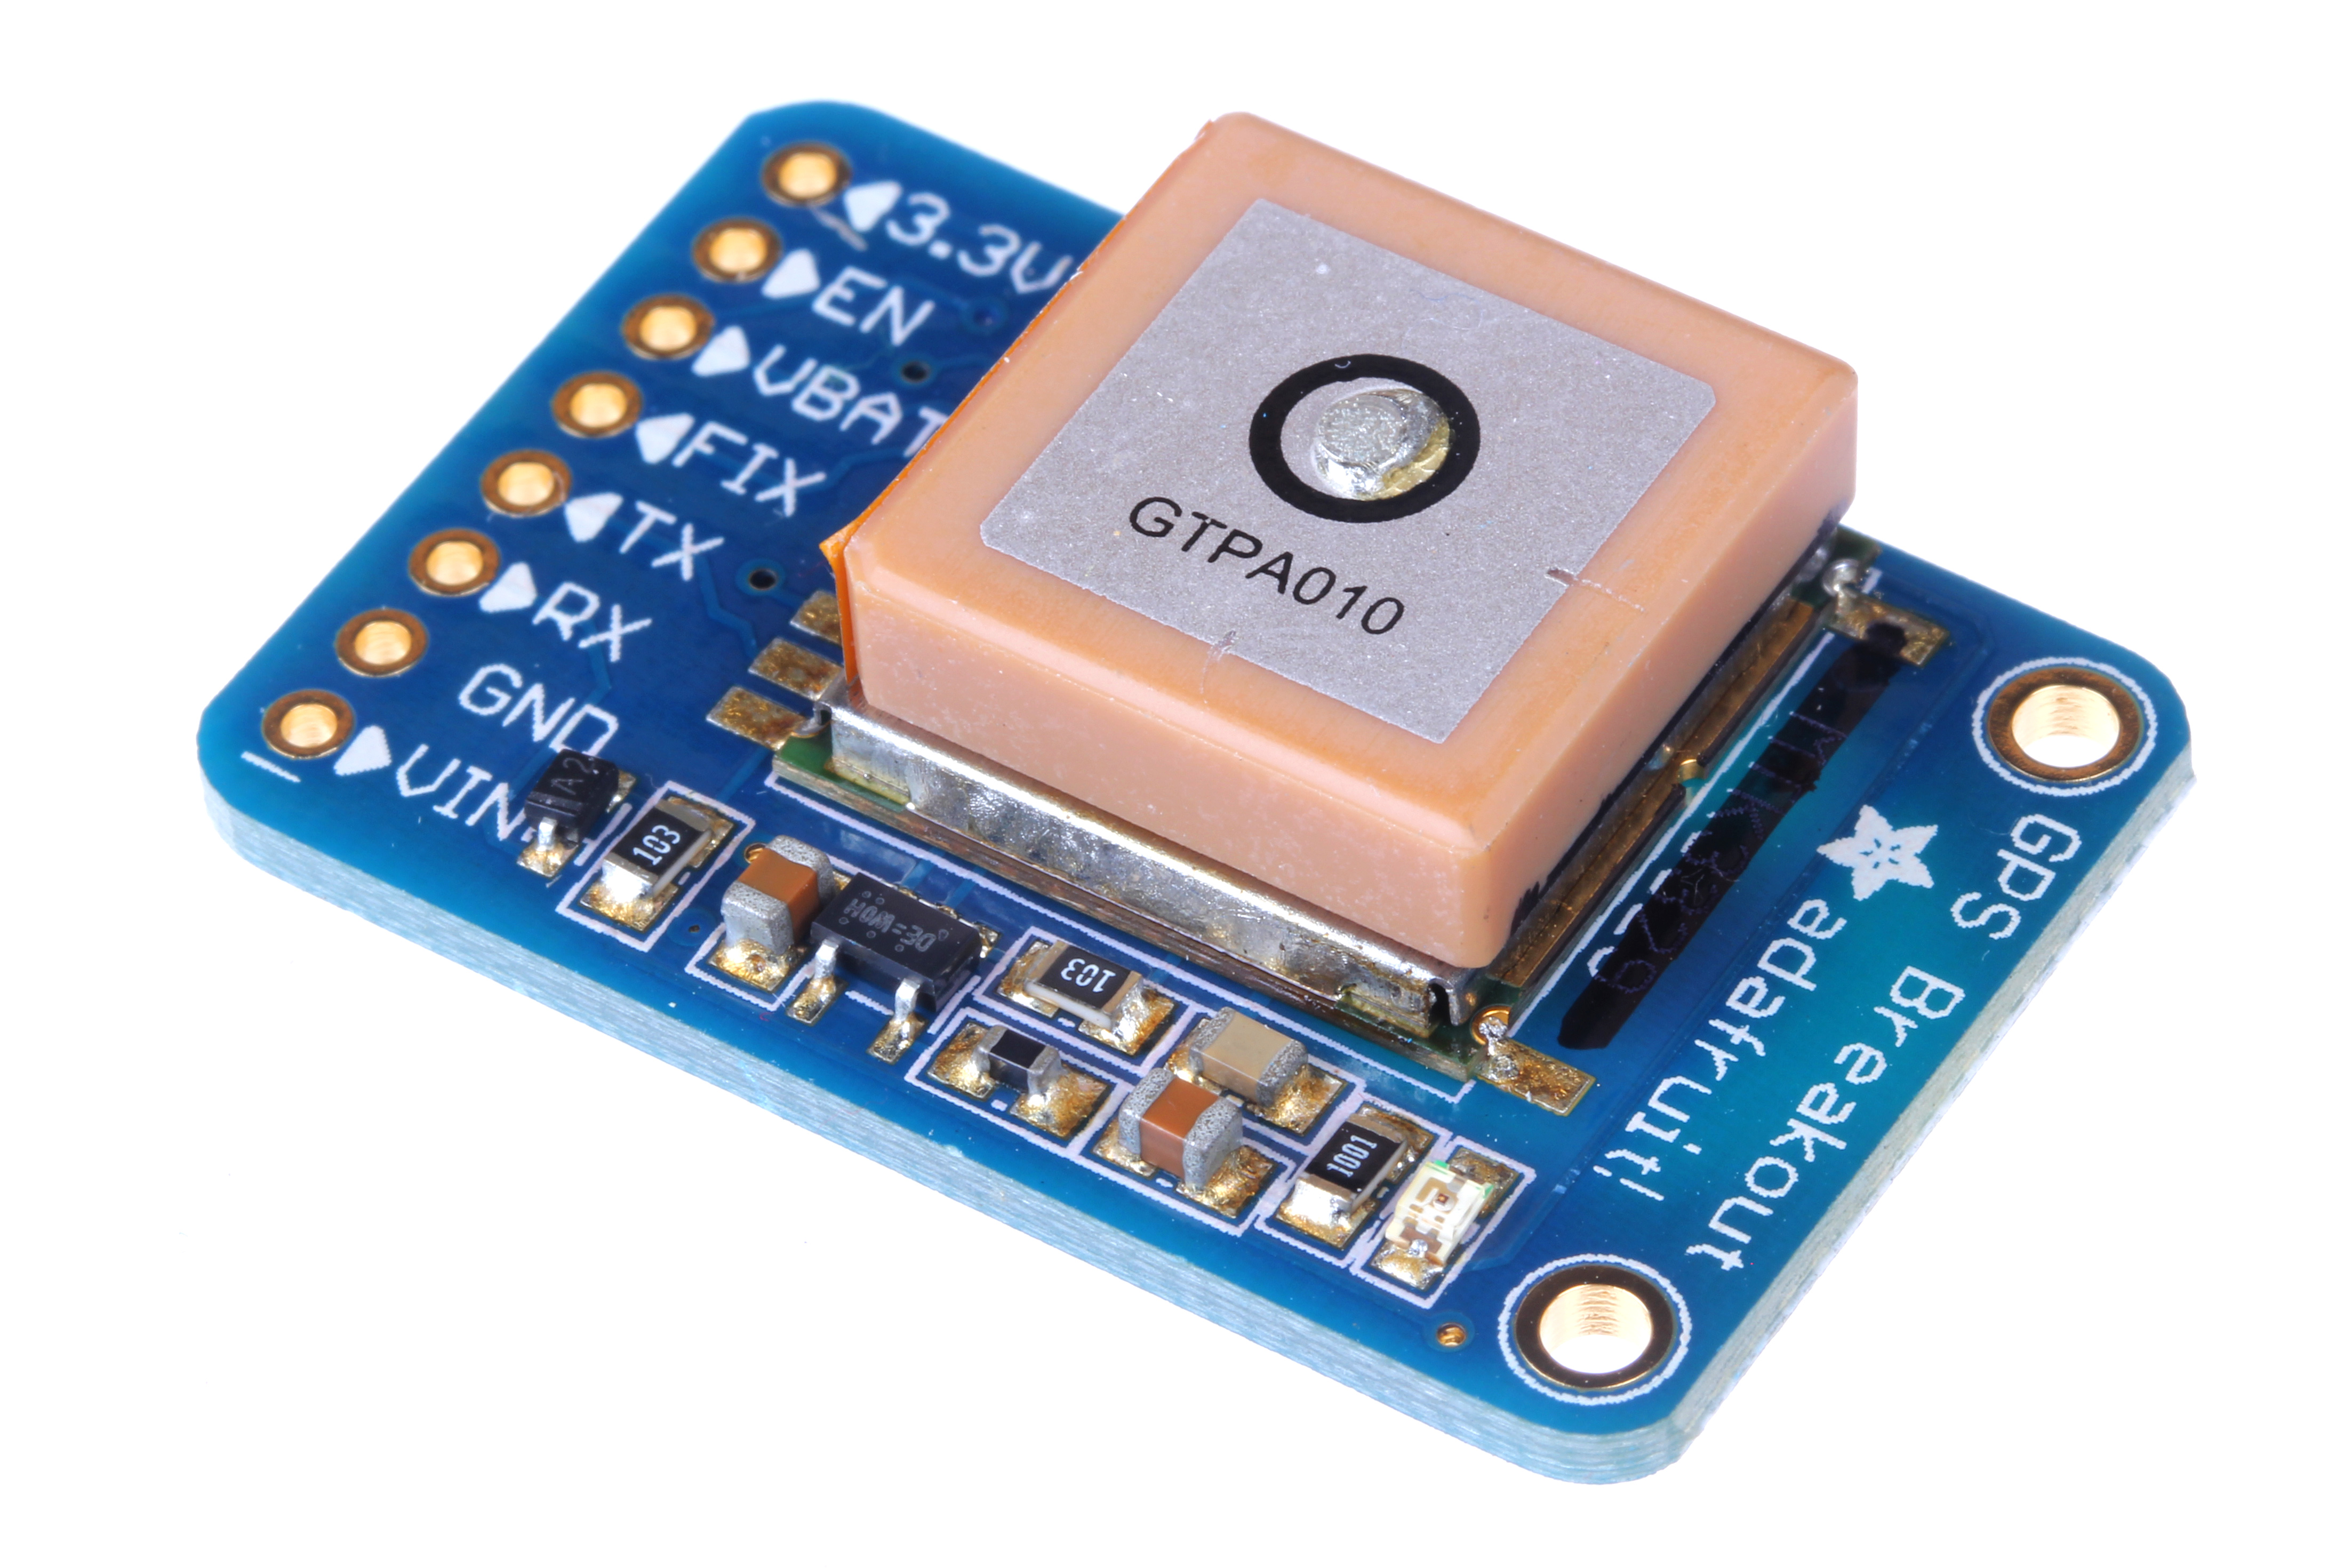
\includegraphics[scale=0.9]{Figures/disp}
\caption[Error del receptor.]{Error del receptor\footnotemark.}
\label{fig:ErrRec}
\end{figure}

\footnotetext{Imagen tomada de: \href{https://upload.wikimedia.org/wikipedia/commons/8/8f/Adafruit_GPS_Module_Breakout.jpg}{https://upload.wikimedia.org/}}

Así como los satélites, los receptores cuentan con sus propios relojes. Debido a costos y dimensiones, éstos no pueden ser atómicos y por tanto son menos exactos, siendo otra fuente de error en la medición.\\

El error asociado a esta causa suele ser de 0.5 metros \citep{fallas2002sistema}.

\subsubsection{Error por Disponibilidad Selectiva}

\begin{figure}[H]
\centering
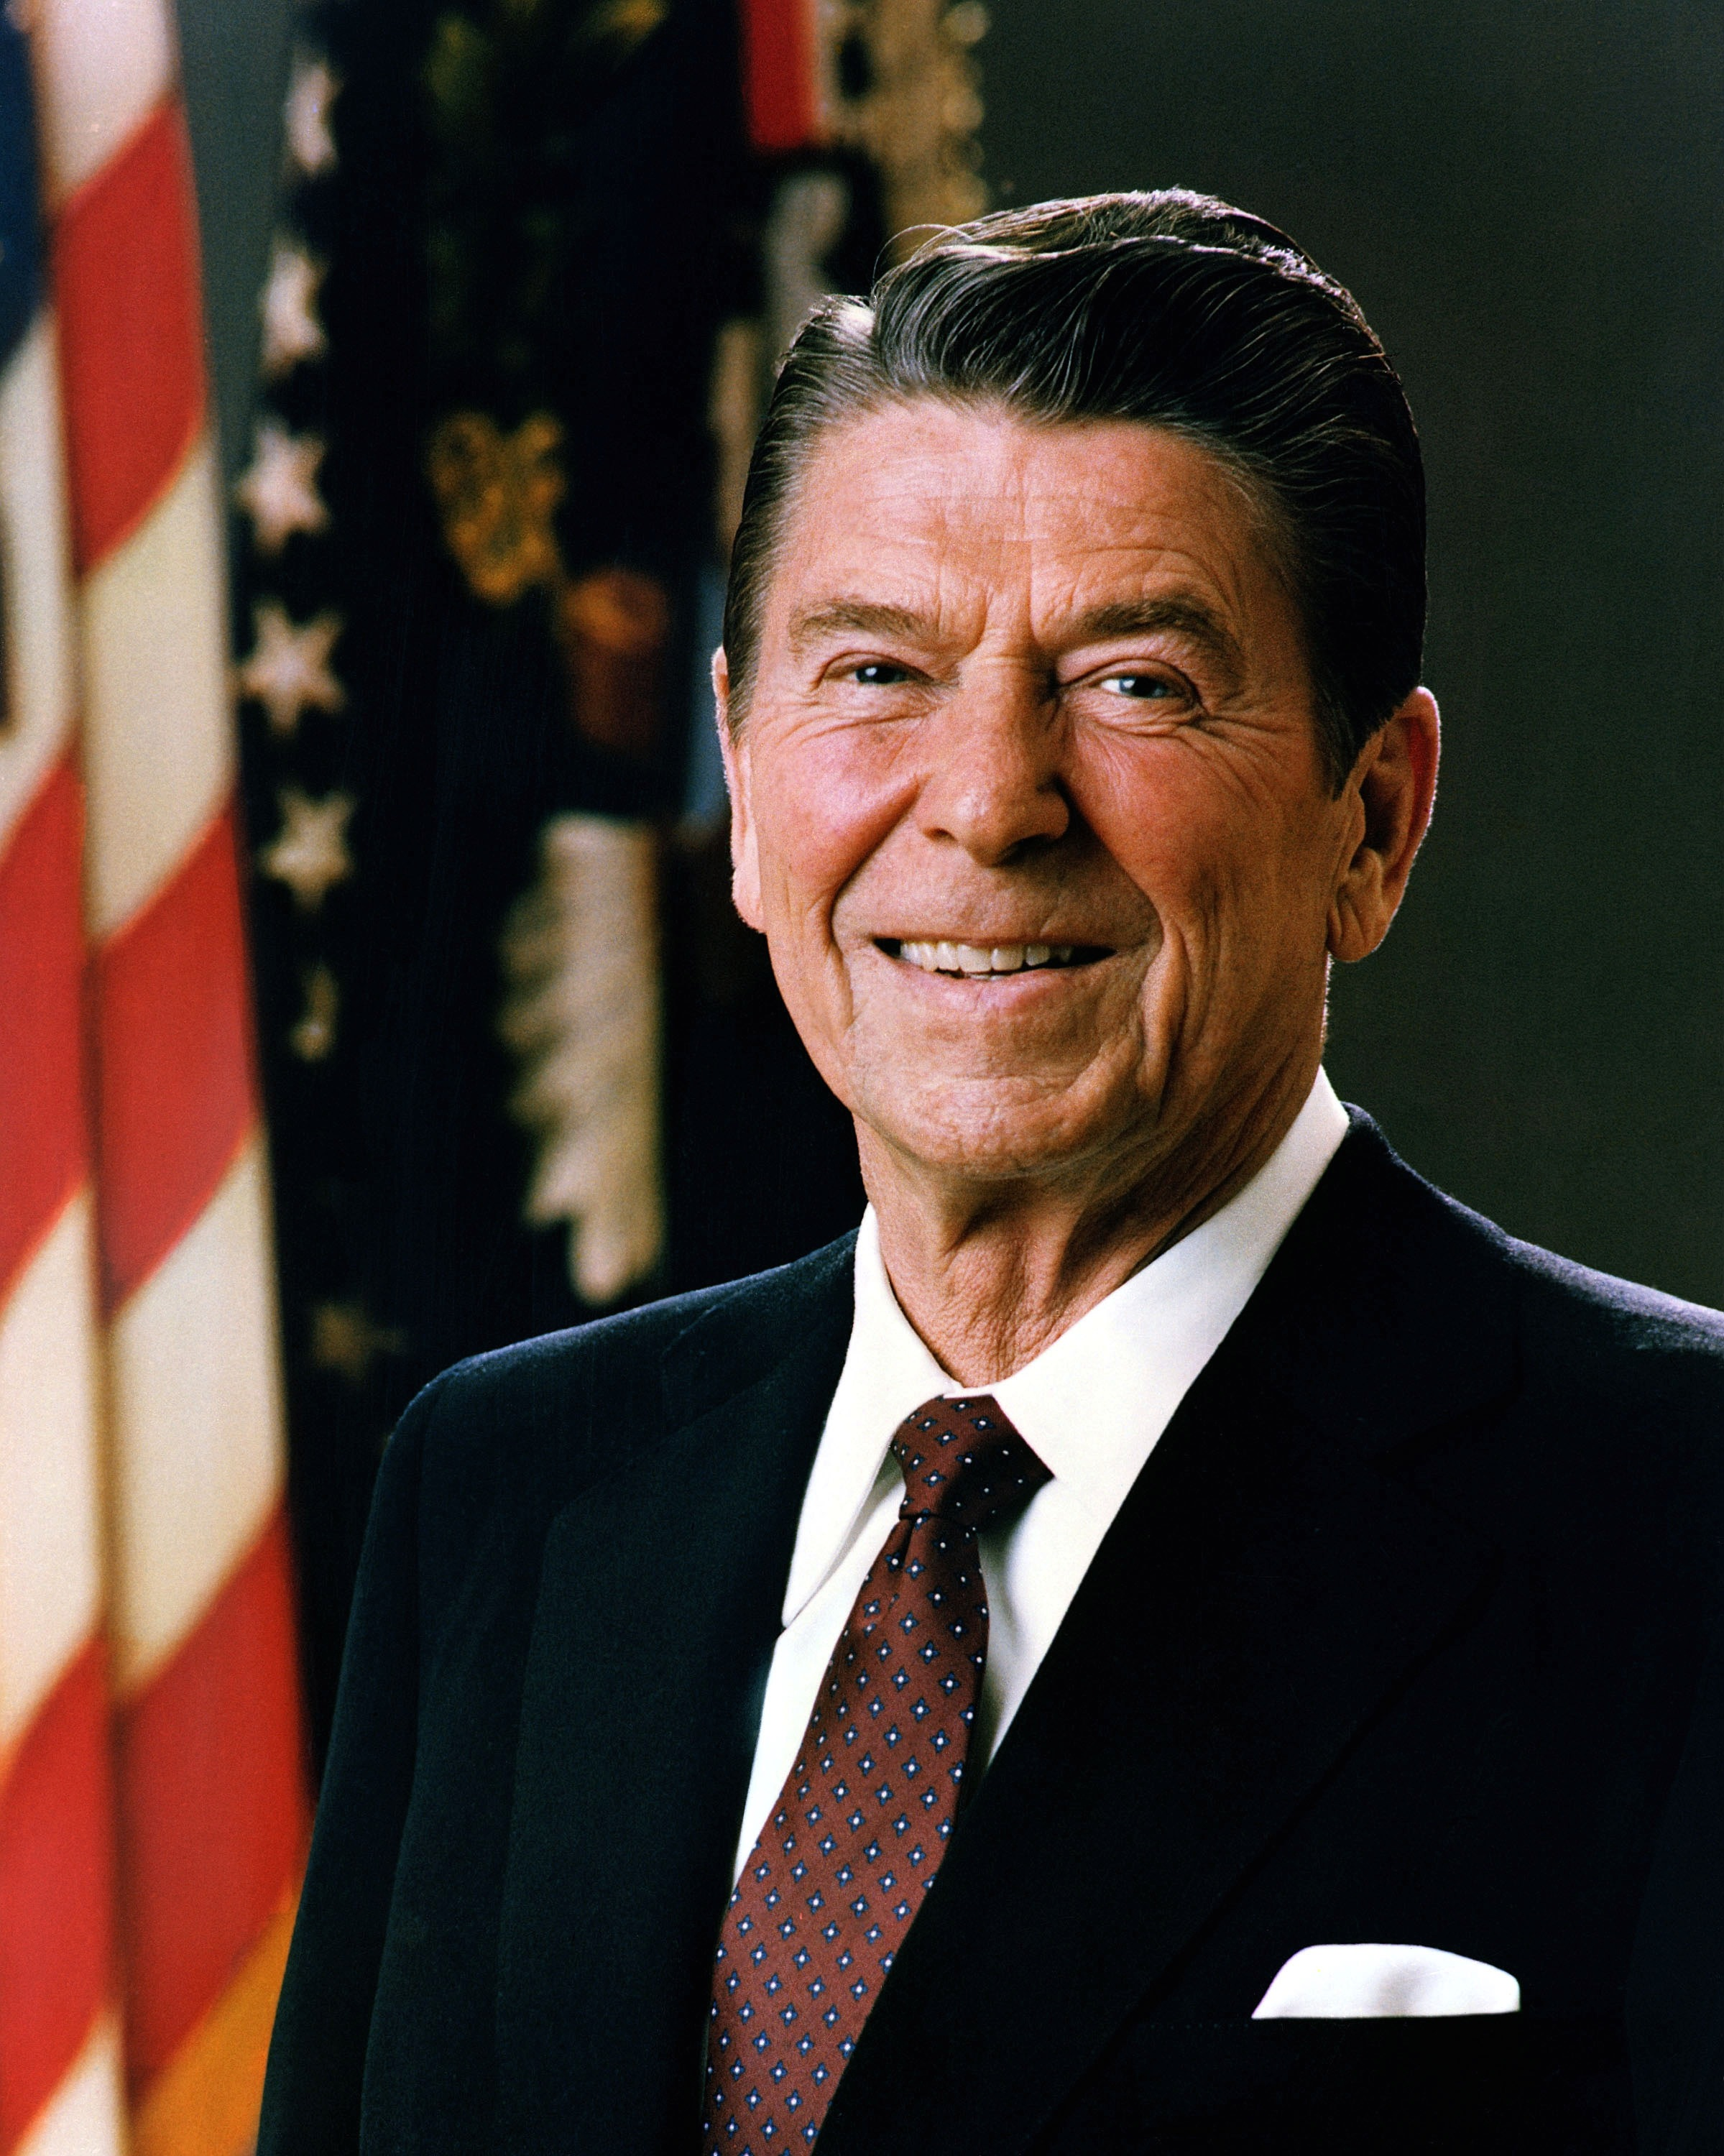
\includegraphics[scale=0.50]{Figures/RonaldReagan}
\caption[Presidente Ronald Reagan.]{Presidente Ronald Reagan\footnotemark.}
\label{fig:ErrDis}
\end{figure}

\footnotetext{Imagen tomada de: \href{https://www.goodfreephotos.com/albums/people/ronald-reagan-portrait-photo.jpg}{https://www.goodfreephotos.com/}}

GPS nació siendo un proyecto de tipo militar. Tras liberarse para uso civil en 1983 por autorización del presidente Ronald Reagan, se habilitaron dos secuencias codificadas llamadas códigos: C/A para uso civil y P para uso militar, con mayor precisión. \\

En el código C/A, se habilitó un error intencionado para evitar un alto grado de precisión, conocido como \textit{Disponibilidad Selectiva}. El presidente Bill Clinton ordenó eliminarle en el año 2000 \citep{termal2014prototipo}.

GPS actualmente mantiene incorporada la opción de disponibilidad selectiva, cuyo error ronda los 100 metros, en caso de que el gobierno de Estados Unidos desee rehabilitarlo. \\

En 2007, el presidente de Estados Unidos anunción que los satélites de los bloques III no incorporarían más dicha opción \citep{chafer2017diseno}.

\section{Comunicación inalámbrica}

\begin{figure}[H]
\centering

\includegraphics[scale=0.30]{Figures/wireless2}
\caption[Símbolo de conectividad inalámbrica.]{Símbolo de conectividad inalámbrica\footnotemark.}
\label{fig:ErrWrl}
\end{figure}

\footnotetext{Imagen tomada de: \href{https://pixabay.com/en/wireless-wi-fi-wireless-signal-1220904/}{https://pixabay.com/}}

Se dice que dos dispositivos se comunican de forma \textbf{inalámbrica} cuando éstos interactúan sin un contacto sólido entre sus masas. \\

En los aparatos electrónicos, se suelen usar ondas de radiofrecuencia, que a su vez se subclasifican dependiendo de la velocidad a la que son emitidas.\\

A menor frecuencia, se obtiene una gran cobertura pero la capacidad se ve mermada. Conforme aumenta, se pierde capacidad de alcance pero la carga de información que puede tener, aumenta. Se dice entonces que existe una relación inversamente proporcional entre capacidad y frecuencia.\\

Actualmente no existe algún organismo internacional que regule las frecuencias utilizadas por los dispositivos de comunicación inalámbrica, por lo que cada país ha de adoptar una regulación propia. En Estados Unidos es la \textit{FCC} (Federal Communications Commission\footnotemark)\footnotetext{Comisión Federal de Comunicaciones, por sus siglas en inglés.}~quien determina dichas regulaciones. Otras organizaciones reguladoras son la \textit{ISO} (International Organization for Standardization\footnotemark) y la \textit{EPCglobal}.

\footnotetext{Organización Internacional para la Estandarización, por sus siglas en inglés.}

La clasificación del uso de las frecuencias por zona geográfica se muestra en el cuadro~\ref{Tab:BandasFreq}.

\begin{table}[H]
\begin{center}
\caption{Bandas de frecuencia en comunicación inalámbrica.}
\label{Tab:BandasFreq}
\begin{tabular}{|l|l|l|l|l|}
	\hline
	\textbf{País/Región} & \textbf{LF} & \textbf{HF} & \textbf{UHF} & \textbf{Microondas}\\
	\hline
	USA & 125-134 KHz & 13.56 MHz & 902-928 MHz & 2400-2483.5 MHz\\& & & & 5725-5850 MHz \\
	\hline
	Europa & 125-134 KHz & 13.56 MHz & 865-868 MHz & 2.45 GHz \\
	\hline
	Japón & 125-134 KHz & 13.56 MHz & No permitida & 2.45 GHz \\
	\hline
	China & 125-134 KHz & 13.56 MHz & No permitida & 2446-2454 MHz \\
	\hline
\end{tabular}
\end{center}
\end{table}

Tanto los sistemas LF y HF son para libre uso en todo el planeta. Sin embargo, UHF necesita de autorización y certificación dependiendo de la zona. En EUA, el uso de UHF no requiere de licencia, pero tiene algunas restricciones \citep{tapia2007identificacion}

\subsection{Protocolo ZigBee}

El estándar IEEE 802.15.4, mejor conocido como ZigBee, es una especificación para aplicaciones de control remoto para cualquier equipo que requiera de un bajo costo y un bajo consumo de potencia en entornos reducidos. ZigBee puede funcionar a tres bandas de frecuencia diferentes: 868 MHz, 915 MHz y 2.4 GHz. \\

\begin{figure}[ht]
\centering
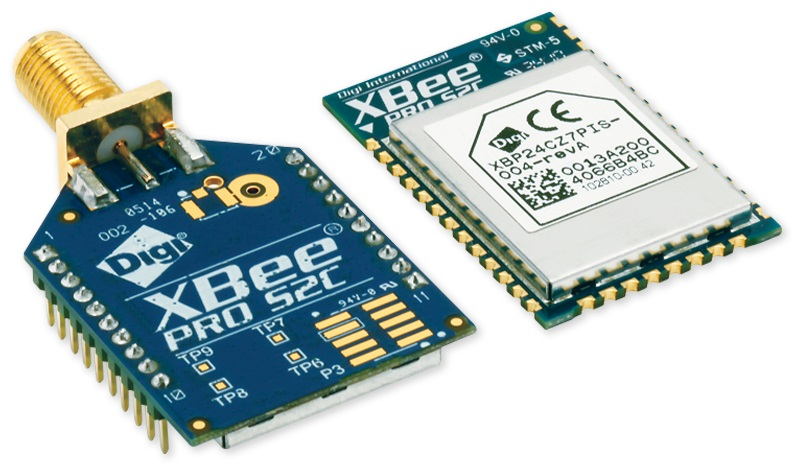
\includegraphics[scale=0.60]{Figures/xbee}
\caption[Equipo XBEE.]{Equipo XBEE\footnotemark.}
\label{fig:XBEE}
\end{figure}

\footnotetext{Imagen tomada de: \href{https://https://www.digi.com/products/xbee-rf-solutions/embedded-rf-modules-modems/xbee-zigbee/product-images/xbee-s2c-zigbee/}{https://www.digi.com/}}

Los módulos XBEE, fabricados por Digi International siguen el protocolo ZigBee. De entre todos esos módulos, destacan los de la serie PRO, ya que poseen una mayor potencia en la señal y en consecuencia, pueden hasta duplicar la capacidad de alcance en la distancia de transmisión. \\

El módulo requiere una alimentación que va desde los 2.8 V hasta los 3.4 V \citep{oyarce2010guia}.

\subsection{Módulo UHF del Ublox C94-M8P GPS}

Los dispositivos GPS Ublox C94-M8P están diseñados para trabajar en pares y vienen incorporados con módulos de comunicación inalámbrica que operan en los 915 MHz de frecuencia en el continente americano. \\

En él, se puede configurar el envío y recepción de diferentes contenidos. El manual de Ublox recomienda usar el formato RTCM3, que será explicado más adelante \citep{ubloxc94}.

\section{Sistemas de cómputo embebidos}

Los Sistemas Embebidos son sistemas programables, que realizan tareas específicas determinadas por el usuario, con el objetivo de optimizar los procesos para mejorar su desempeño y eficiencia, reduciendo tamaño y costos de producción. \\

Se caracterizan por el bajo consumo de energía. Está compuesto por tres componentes principales: Procesador, Dispositivos de almacenamiento y Periféricos \citep{caballero2014desarrollo}.

\subsection{BeagleBone Black}

\begin{figure}[ht]
\centering
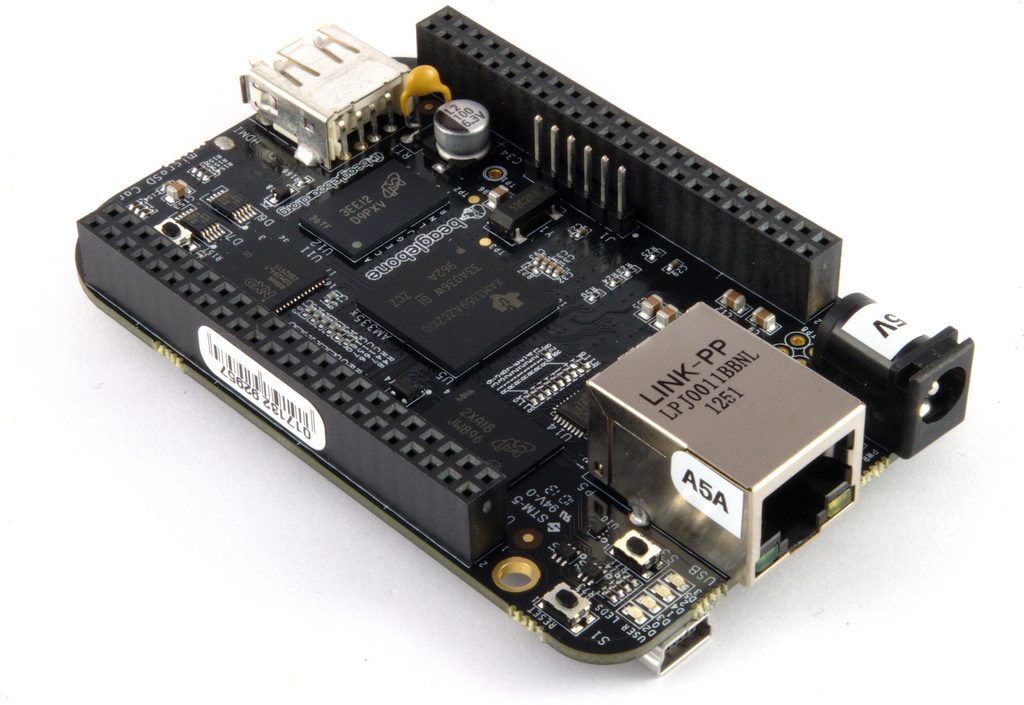
\includegraphics[scale=0.36]{Figures/BeagleBoneBlack}
\caption[BeagleBone Black.]{BeagleBone Black\footnotemark.}
\label{fig:BBlack}
\end{figure}

\footnotetext{Imagen tomada de: \href{https://www.flickr.com/photos/120586634@N05/14491195107}{https://www.flickr.com/}}

La BeagleBone es una plataforma de desarrollo de bajo costo. \\

Desarrollada por la BeagleBone Foundation de los Estados Unidos, una fundación sin ánimos de lucro, cuyo objetivo es la promoción de hardware y software de código abierto para el desarrollo de sistemas embebidos. \\

Por su diseño, posee una arquitectura ARM, que posee soporte de varias distribuciones Linux \citep{coronado2014desarrollo}. \\

Por su condición de hardware y software abierto, tanto sus esquemáticos del hardware, como las códigos fuente de su software están disponibles a todos los usuarios. \\

De las ventajas que posee una arquitectura como la del BeagleBone, basada en microprocesadores, es que su uso conduce a plataformas más poderosas, capaces de realizar tareas de gran carga computacional \citep{coley2013beaglebone}.

\subsection{BlackLib}

BlackLib es una biblioteca que permite controlar el hardware y los puertos de la BeagleBone Black a través del lenguaje C++. Puede leer entradas análogas, generar señales pwm, usar pines de propósito general o GPIO, y comunicarse con otros dispositivos a través de comunicación serial \citep{blacklib}.

\section{Software Libre}

\begin{figure}[H]
\centering

\includegraphics[scale=0.15]{Figures/opens}
\caption[Logotipo de Open Source Initiative.]{Logotipo de Open Source Initiative\footnotemark.}
\label{fig:opens}
\end{figure}

\footnotetext{Imagen tomada de \href{https://upload.wikimedia.org/wikipedia/commons/thumb/4/42/Opensource.svg/2000px-Opensource.svg.png}{https://upload.wikimedia.org/}}

El \textbf{software} es un conjunto de instrucciones en lenguaje máquina para que una computadora realice funciones específicas.\\

El código máquina llega a través de un código más entendible para humanos, llamado código fuente, que un compilador se encarga de traducir a lenguaje máquina. Cuando el código fuente no es accesible para nadie, se dice que se trata de código cerrado \citep{i2005software}.\\

El software libre es aquél cuyo código fuente puede ser usado, copiado, estudiado, modificado y redistribuido libremente. A pesar de dicha capacidad de propagación del código, el software puede seguir siendo vendido comercialmente \citep{garcia2007promocion}. 

\subsection{GNU/Linux}
Linux es un sistema operativo. Un sistema operativo es un conjunto de programas que permiten la interacción con el hardware, además de ejecutar otros programas, así como crear una interfaz con el usuario. En un sistema GNU/Linux, Linux es el núcleo o kernel, y GNU es el conjunto de programas \citep{debian}. 


\section{Real Time Kinematics}

\begin{figure}[H]
\centering
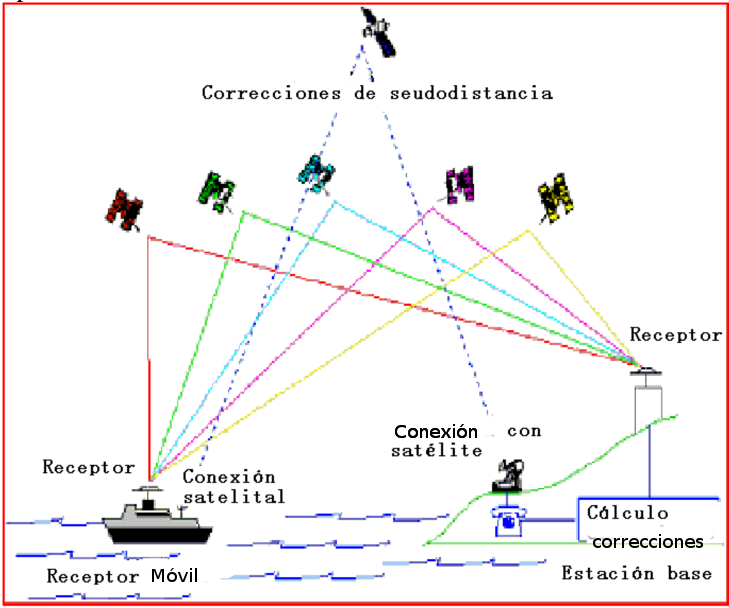
\includegraphics[scale=0.53]{Figures/DGPS1}
\caption[Esquema de funcionamiento en RTK.]{Esquema de funcionamiento en RTK, por \cite{fallas2002sistema}.}
\label{fig:RTK}
\end{figure}

Se le llama Sistema de Navegación Cinética Satelital en Tiempo Real (RTK, Real Time Kinematics por sus siglas en inglés), a las correcciones de la señal del GPS basadas en las señales L1 y L2. \\

Todo está en torno al siguiente supuesto: \\

Se tienen dos receptores a una distancia de pocos km entre sí. En esta condición, se podría esperar que los errores causados por el reloj atómico del satélite, por la ionósfera y la tropósfera afectarían de igual manera y con la misma magnitud a ambos receptores, por su proximidad. Si la posición exacta de uno de los receptores es conocida, entonces esta información puede ser usada para determinar el error asociado a las lecturas de dicho receptor y después aplicar la corrección al otro dispositivo. \\

Al GPS cuya posición es conocida recibe el nombre de \textbf{receptor base} y el segundo es llamado \textbf{receptor móvil}. La estación base calcula la distancia entre cada uno de los satélites de los que recibe señal y su posición (también conocida) para determinar el error asociado a la medición de distancia. Esa información la envía al receptor móvil, quien aplica la corrección hacia dicho satélite, obteniendo así un conocimiento más exacto sobre su posición \citep{fallas2002sistema}. \\

Con todas las correcciones aplicadas de forma ideal, se alcanza una precisión mejor a los 10 cm \citep{cerrato2011diseno}. \\

Conforme el receptor móvil se aleja gradualmente de la estación base, gradualmente, la utilidad de las correcciones proporcionadas de la segunda a la primera, disminuye \citep{mueller1994networked}.

\section{Formato RTCM-3}

Este formato es un estándar internacional para transmitir datos de posicionamiento en tiempo real. \\

Es utilizado sólo por las estaciones base para proporcionar sus observaciones. \\

Su estructura consiste en un mensaje de 42 bits fijos más otros bits que pueden variar de acuerdo al o los mensajes que se requiera enviar \citep{rubinov2011review}, como muestra el cuadro~\ref{Tab:RTCM-Struct}.\\

\begin{table}[!htb]
\begin{center}
\caption{Estructura del mensaje RTCM-3.}
\label{Tab:RTCM-Struct}
\begin{tabular}{|l|l|l|l|l|}
	\hline
	\textbf{\small Preámbulo}& \textbf{\small Reservado}& \textbf{\small Tamaño del mensaje}& \textbf{\small Datos del mensaje}& \textbf{\small Checksum}\\
	\hline
	8 bits & 6 bits & 10 bits & n bits & 24 bits \\
	\hline
	0xD3 & \parbox[t]{1.9cm}{Sin definir} & \parbox[t]{2.9cm}{Tamaño del mensaje en bytes} & \parbox[t]{2.9cm}{Tamaño variable en bytes} & \parbox[t]{2.05cm}{Definición QualComm CRC-24Q}\\
	\hline
\end{tabular}
\end{center}
\end{table}

El mensaje utilizado en este trabajo contendrá los siguientes datos: \\

\begin{table}[!htb]
\begin{center}
\caption{Contenido del mensaje en formato RTCM-3.1}
\begin{tabular}{|l|}
	\hline
	\textbf{Mensaje RTCM-3.1}\\
	\hline
	\tabitem \textbf{1005:} (X,Y,Z) Coordenadas fijas de la antena. \\
	\tabitem \textbf{1077:} Observaciones de GPS. \\
	\tabitem \textbf{1087:} Observaciones de GLONASS.\footnotemark \\
	\hline
\end{tabular}
\end{center}
\end{table}

\footnotetext{Homólogo ruso del sistema americano GPS.}

\section{RTKLIB}

\begin{figure}[H]
\centering

\includegraphics[scale=1.8]{Figures/rtklib}
\caption[Logotipo de RTKLIB.]{Logotipo de RTKLIB\footnotemark.}
\label{fig:rtklib}
\end{figure}

\footnotetext{Imagen tomada de \href{https://avatars3.githubusercontent.com/u/4287338?v=3&s=400}{https://avatars3.githubusercontent.com/}}

Desarrollado por Tomoji Takasu, RTKLIB es un paquete de programas de código abierto escrito en C, para posicionamiento tanto estándar como preciso con sistemas de bajo costo. Soporta varios modos de posicionamiento tales como: Simple, Diferencial, Cinemático, entre otros. \\

En todos sus modos soporta tanto procesamiento en tiempo real así como postprocesamiento \citep{takasu2009development}.

\subsection{Modos de funcionamiento}

RTKLIB puede funcionar en distintos modos. Se explicarán un par de ellos en conformidad con su relevancia en este proyecto:

\begin{itemize}
\item Modo estático.
\item Modo cinemático.
\end{itemize}

RTKLIB utiliza un filtro de Kalman extendido (\textit{EKF}, extended Kalman filter, por sus siglas en inglés), para obtener los resultados de sus cálculos de aproximación. 

\subsubsection{Modo estático}
En este modo es necesaria una larga observación del cielo y de recolección de datos. Este requisito está fundamentado dado el cambio en la geometría del trayecto de los satélites, que apoyan en la resolución de ambigüedades \citep{wisniewski2013evaluation}.

\subsubsection{Modo cinemático}
Requerido cuando el objeto al que se quiere conocer su posición, se encuentra en movimiento. Permite obtener decímetros de precisión. Para un funcionamiento óptimo, necesita las coordenadas de una estación base conocida en el archivo de configuración. Los datos de esta estación fija pueden ser obtenidos mediante mensajes RTCM \citep{wisniewski2013evaluation}.

\section{Vehículos aéreos no tripulados - VANT}

\begin{figure}[H]
\centering
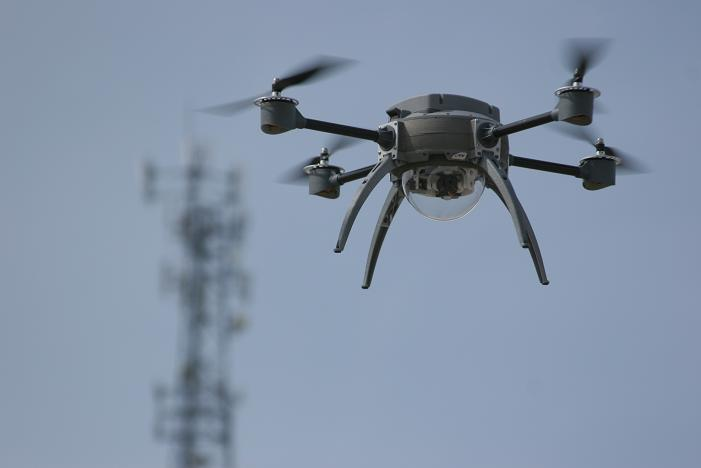
\includegraphics[scale=0.75]{Figures/UAV}
\caption[Vehículo aéreo no tripulado.]{Vehículo aéreo no tripulado\footnotemark.}
\label{fig:UAV}
\end{figure}

\footnotetext{Imagen tomada de \href{https://upload.wikimedia.org/wikipedia/commons/7/79/Aeryon_Scout_In_Flight.jpg}{https://upload.wikimedia.org/}}

Los vehículos aéreos no tripulados (\textit{VANT} o \textit{UAV}, Unmanned Aerial Vehicle por sus siglas en inglés) estuvieron orientados inicialmente para operaciones de contexto militar \citep{fahlstrom2012introduction}.\\

Un VANT es definido como un vehículo con operaciones y sistemas mecatrónicos, con computadoras a bordo y supervisado por humanos desde tierra \citep{haluani2015tecnologia}.\\

En usos civiles, se pueden destacar empresas que investigan formas de entregar paquetes mediante el uso de esta tecnología, así como observaciones meteorológicas.\\

Algunas áreas de aplicación son \citep{addati2014introduccion}:

\begin{itemize}
\item Imágenes y vídeo aéreo.
\item Monitoreo y vigilancia.
\item Inspección de infraestructuras.
\item Búsqueda y rescate.
\item Gestión de emergencias.
\item Mapeo de terrenos.
\end{itemize}

\subsection{Instrumentación de vuelo}

La instrumentación de vuelo es la encargada de obtener el estado de vuelo del UAV de manera precisa, así como el entorno en el que se encuentra haciendo uso de distintos sensores.\\

Dependiendo de la finalidad de una misión de vuelo, se pueden encontrar los siguientes sistemas de sensado \citep{barrientos2007vehiculos}:\\

Para un marco de referencia inercial.
\begin{itemize}
\item Acelerómetros.
\item Giroscopios.
\end{itemize}
Para posicionamiento y velocidad.
\begin{itemize}
\item GPS.
\item Compás.
\end{itemize}

\section{Conclusión}

Tras una revisión de los conceptos y componentes necesarios, se procede a continuación a detallar la forma en cómo cada uno de ellos conforma un elemento clave para la obtención del objetivo.\\

En el capítulo \ref{Chap:DisHard}, se habla acerca de la integración de los componentes descritos en el capítulo \ref{Chap:Marco}. Se presentan descripciones acerca de los componentes, fotografías, especificaciones de funcionamiento y modos de operación, así como las condiciones de uso para un correcto desempeño.  
% Chapter 2

\chapter{Diseño del hardware}
\label{Chap:DisHard} % For referencing the chapter elsewhere, use \ref{Chapter2} 

%----------------------------------------------------------------------------------------

\section{Introducción}

Lorem ipsum dolor...

\section{Prototipo}

La interconexión general del sistema quedará como sigue: Es posible observar a la estación base o de tierra en la parte inferior izquierda de la imagen. La estación móvil o Rover se encontrará navegando libremente en un espacio cercano en función a la potencia de los módulos de radiofrecuencia usados para comunicar a ambas plataformas.

\section{Descripción del funcionamiento}

A la estación base se le asignará un conjunto de coordenadas fijas de latitud, longitud y altura sobre el nivel del mar, que es donde ella deberá ser colocada. El GPS realizará las triangulaciones necesarias para obtener su posición estimada, también en coordenadas, a través de los satélites. Así, comparando a las coordenadas previamente fijadas de su posición exacta con las obtenidas de las triangulaciones, la estación base calculará el
error que existe en ese instante en las mediciones y procederá a informar, mediante los módulos de comunicación de radiofrecuencia, a la estación móvil, para que proceda a hacer las correcciones necesarias y obtener una aproximación depurada de su posición y sus movimientos. \\

Se realizó un experimento que consistió en trazar y seguir una determinada ruta para poder observar las diferencias entre un sistema RTK y uno con el GPS triangulando por sí solo. \\

También fueron colocadas marcas en el suelo para poder tener una guía precisa del camino a seguir y repetir en ambos experimentos. \\

Se usaron las coordenadas que Google Maps proporciona, como referencia. De este modo, los resultados irán conforme a los mapas de este servicio. \\

Al final, la ruta a seguir quedaría de este modo:

\section{Descripción del experimento}

Lorem ipsum dolor...

\section{Conclusión}

Lorem ipsum dolor...

En el capítulo siguiente...
% Chapter 2

\chapter{Resultados} % Main chapter title

\label{Chap:Res} % For referencing the chapter elsewhere, use \ref{Chapter2} 

\section{Introducción}

En este capítulo se presentarán los procedimientos requeridos para llevar a cabo el experimento descrito en el capítulo anterior, y se expondrán los resultados obtenidos de realizar las mediciones. Posteriormente, se mostrarán gráficas de los datos obtenidos con una explicación de sus componentes y su respectiva interpretación. \\

\section{Dibujo del plano}

Para el trazo de la figura cuadrado, que será de 15 metros por lado, se utilizaron dos varas unidas por una fracción de rafia como las de la figura~\ref{fig:HerTraz}, utilizados para el trazado de las circunferencias necesarias.\\

\begin{figure}[H]
\centering
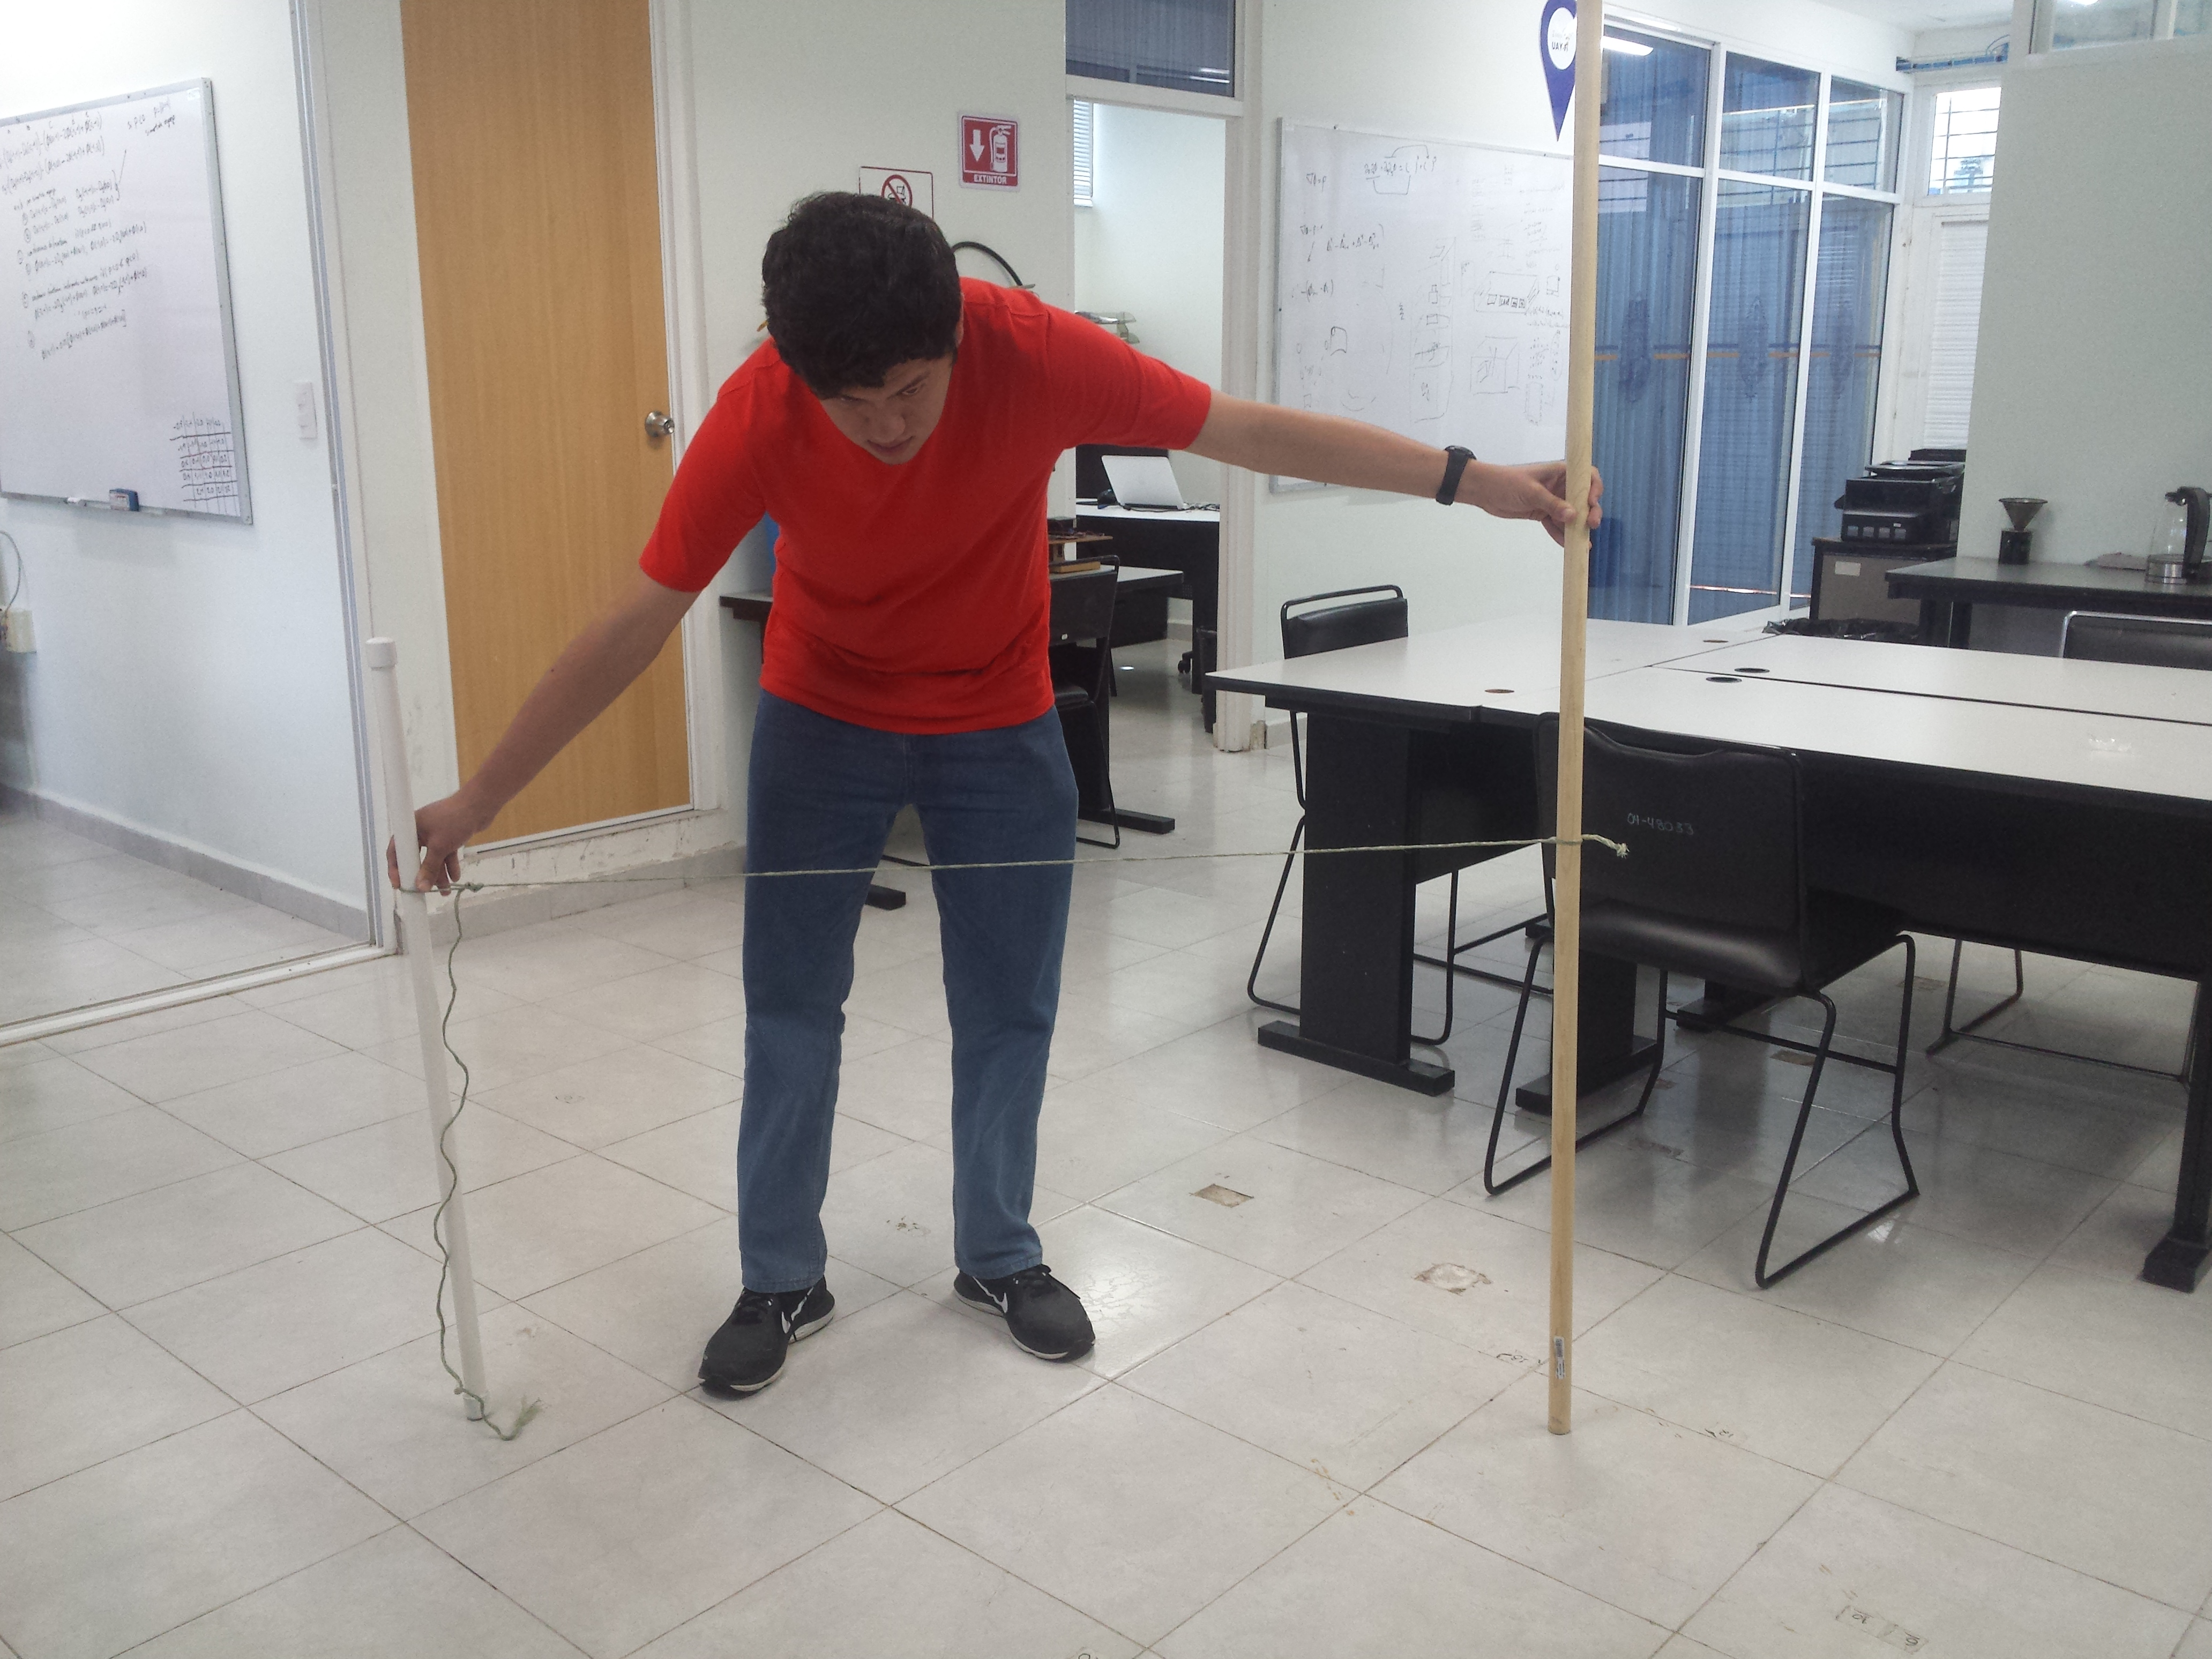
\includegraphics[width=0.95\textwidth]{Figures/Herr}
\caption[Herramientas de trazado.]{Herramientas de trazado.}
\label{fig:HerTraz}
\end{figure}

Para garantizar que se trace una línea recta en cada uno de los lados de la figura, se utilizó una cuerda de nailon de 17 metros de longitud, que una vez tensa, permitió realizar las marcas equidistantes cada 3 metros con un flexómetro, signos en el suelo como los de la figura~\ref{fig:MarEq}.

\begin{figure}[H]
\centering
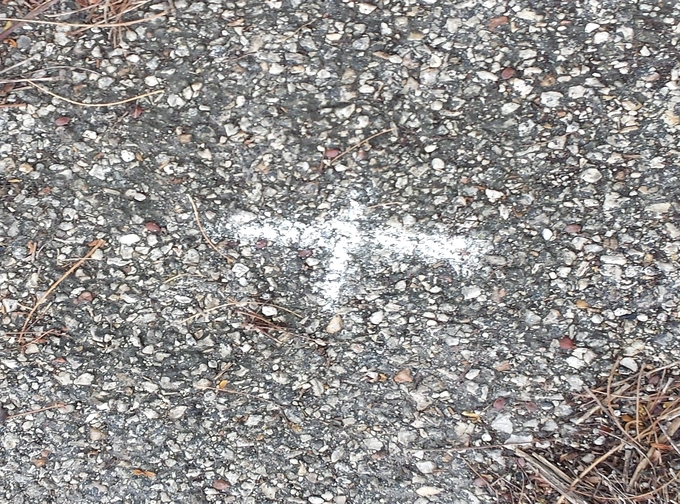
\includegraphics[width=0.95\textwidth]{Figures/Equid}
\caption[Marcas equidistantes en el suelo.]{Marcas equidistantes en el suelo.}
\label{fig:MarEq}
\end{figure}

\section{Mediciones}

\begin{figure}[H]
\centering
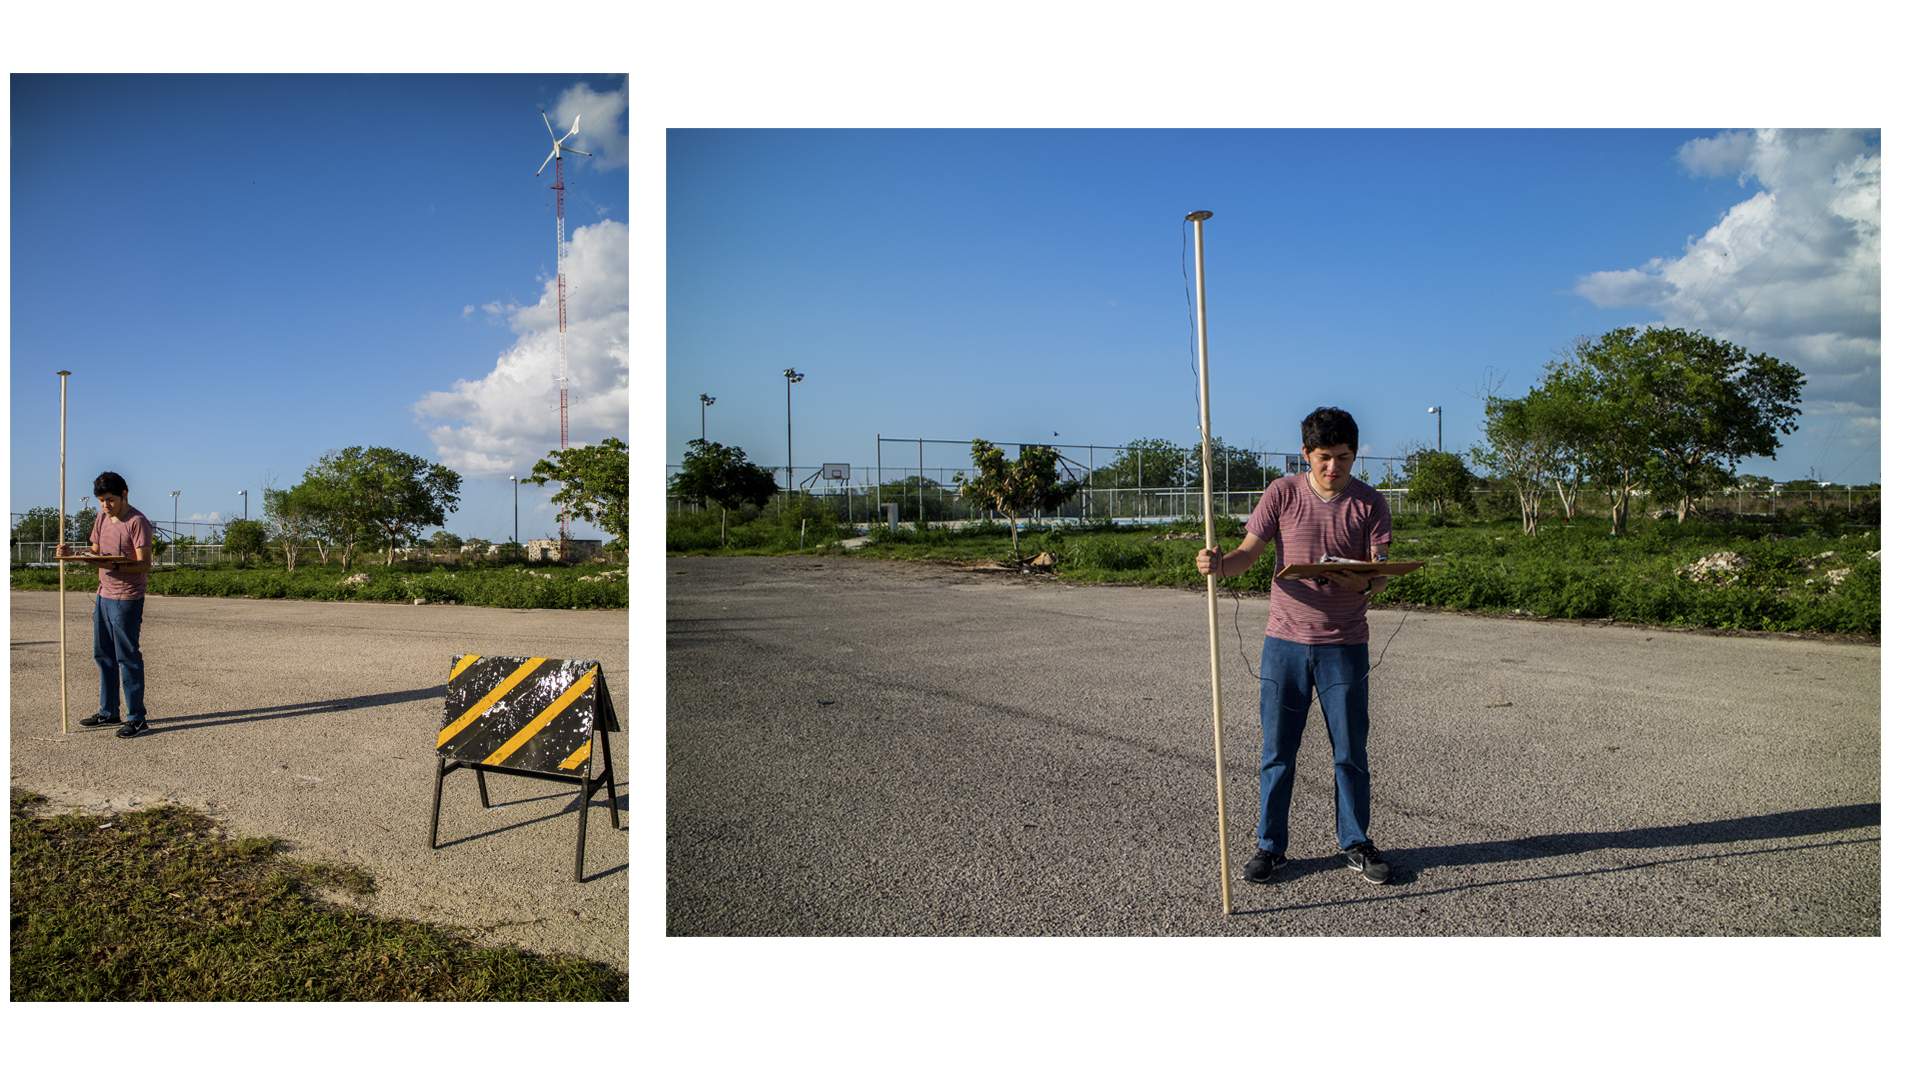
\includegraphics[width=0.95\textwidth]{Figures/22jpg}
\caption[Toma de muestras de coordenadas.]{Toma de muestras de coordenadas.}
\label{fig:Medc}
\end{figure}

Una vez finalizada la separación en 5 segmentos por cada lado de la figura, de 3 metros de separación entre ellos, se obtienen 6 puntos de medición; tras ser configuradas ambas estaciones, se procedió a realizar las mediciones de las coordenadas en los puntos. En la figura~\ref{fig:Medc} se muestran diversos momentos de la toma de muestras correspondientes a las mostradas en este capítulo. Puede observarse un cielo en su mayor parte despejado. Se decidió tomar muestras tanto en el modo Real-Time Kinematics como con el modo de un solo GPS sin retroalimentación de una estación base para comparar resultados. En ambos modos, se recorrió el trazado de la figura dos veces con la antena, en dos sentidos diferentes, llegando a obtener dos mediciones de coordenadas por punto en cada modo de funcionamiento.\\

\begin{figure}[H]
\centering
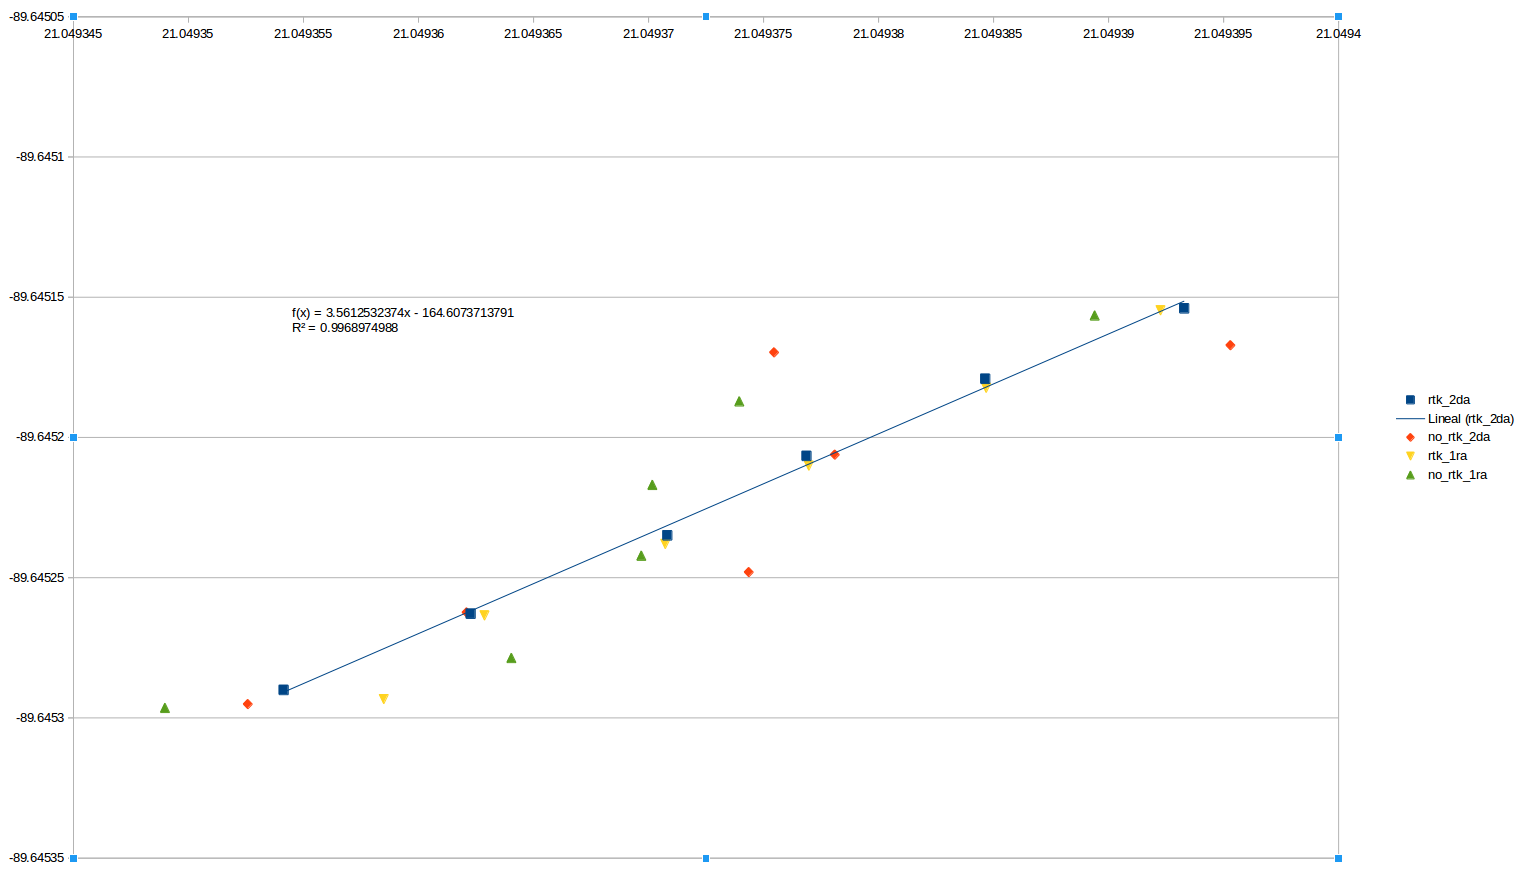
\includegraphics[width=1\textwidth]{Figures/Dispers}
\caption[Diagrama de dispersión de datos registrados en las marcas del lado sur de la figura.]{Diagrama de dispersión de coordenadas registradas en las marcas del lado sur de la figura.}
\label{fig:Disp}
\end{figure}

En la figura~\ref{fig:Disp} se comparan las mediciones realizadas en las marcas del lado sur de la figura, mediante una regresión lineal utilizando los puntos del segundo recorrido en el modo Real-Time Kinematics. Los cuadrados azules marcan el segundo recorrido de muestreo de la figura realizado en el modo Real-Time Kinematics. Los triángulos amarillos marcan las muestras del primer recorrido de muestreo en el mismo modo. El rombo rojo y el triángulo verde marcan el mismo orden pero del modo con un sólo GPS sin retroalimentación de posicionamiento.\\

\newpage

Las muestras realizadas en el modo Real-Time Kinematics muestran, en su segundo recorrido, marcado con cuadros azules, un mayor ajuste a la línea recta de la figura, donde el valor del coeficiente de correlación múltiple $R^{2} \approx 0.997$\footnotemark sugiere un alto ajuste a una línea recta. En el primer recorrido, marcado con triángulos amarillos, se puede observar la misma tendencia pero con un menor ajuste. El resto de puntos, marcados con círculos rojos y triángulos verdes, son en un modo sin Real-Time Kinematics y se puede observar que el ajuste a una línea recta es mucho menor que el modo RTK, llegando a tener variaciones bastante considerables respecto a dicho método.\\

\footnotetext{El valor de $R^{2}$ varía de 0 a 1. Mientras más cerca esté su valor de la unidad, se sugiere una correlación más alta a la recta en este caso. Las muestras escogidas para realizar este cálculo fueron las que se realizaron con Real-Time Kinematics durante la segunda vuelta.}

En el modo Real-Time Kinematics, en cada muestra, existe un valor denominado \textit{ratio} que indica la calidad de la señal de los satélites y de las mediciones del GPS en el \textit{rover} de forma proporcional. En otras palabras, mientras más alto sea el valor de ratio, mucha mejor será la corrección de la señal de GPS. En la figura~\ref{fig:Ratio} se observa cómo en las primeras muestras, el valor del \textit{ratio} oscilaba en valores bajos (se consideran valores bajos aquellos que están debajo de 3). Conforme el tiempo avanzaba, se captaban más satélites y, como consecuencia, el valor del \textit{ratio} ascendió a valores altos. Este comportamiento se ajusta a la gráfica de dispersión en la figura~\ref{fig:Disp}, que muestra que en el primer recorrido, denotado con un triángulo amarillo, el primer punto muestreado (el que está más a la izquierda) estuvo algo más separado de la recta que el resto de muestras en el mismo modo de funcionamiento.

\begin{figure}[H]
\centering
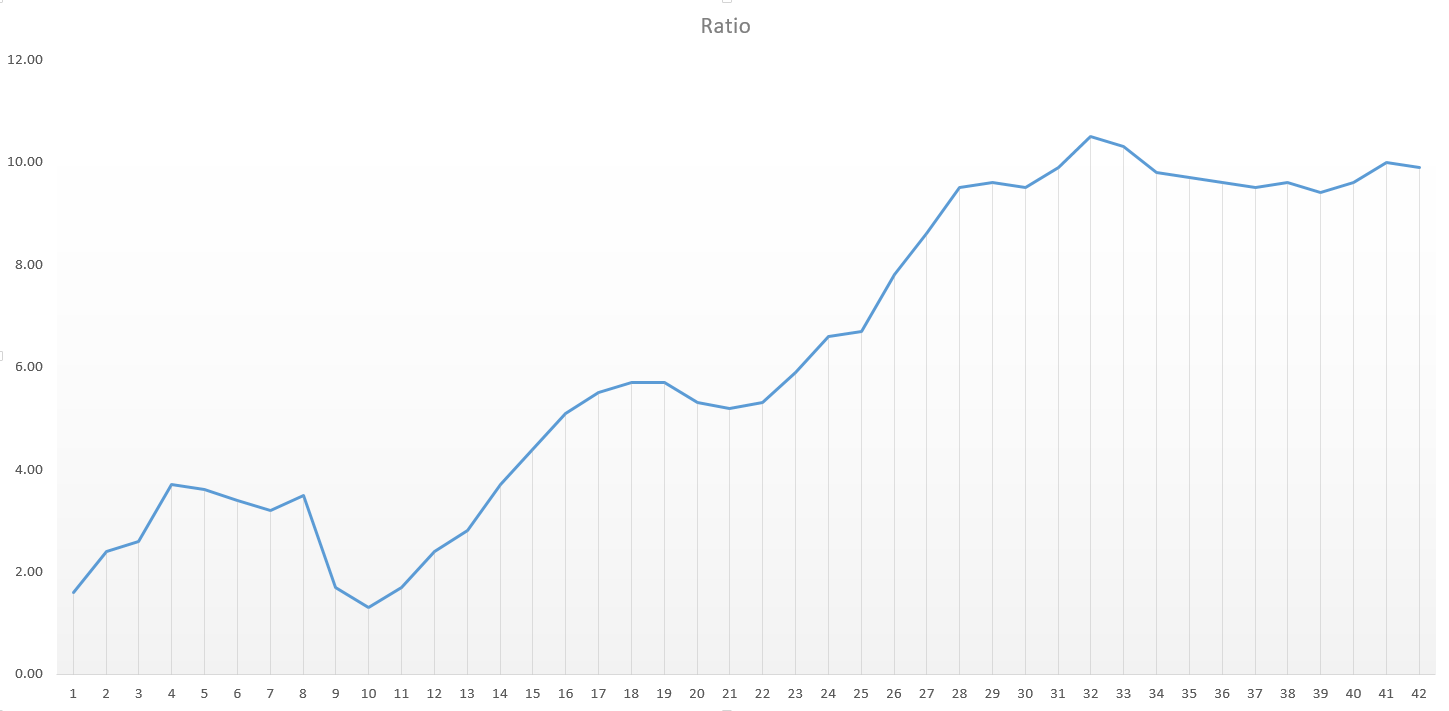
\includegraphics[width=1\textwidth]{Figures/Ratio}
\caption[Gráfica del ratio (confianza de los datos presentados).]{Gráfica del ratio (confianza de los datos presentados).}
\label{fig:Ratio}
\end{figure}

Para obtener el error en metros de las mediciones, se calculó la diferencia existente en distancia entre dos puntos marcados para realizar muestras de coordenadas correspondientes al mismo lado del cuadrado. Todas las coordenadas tomadas para estos cálculos son los correspondientes a la segunda vuelta de cada modalidad. El punto de origen fue el vértice inferior izquierdo y las distancias fueron tomadas en el sentido de las agujas del reloj. Así, el segmento 1 corresponderá a la distancia entre el origen, y el primer punto a 3 metros de él que se ubica en el lado izquierdo de la figura. El segmento 2 corresponderá a la distancia entre el primer y segundo punto en el lado izquierdo del cuadrado, y así sucesivamente. Cada par de puntos deben tener una diferencia existente de tres metros entre sí. Por tanto, se calculó la diferencia en metros a partir de las coordenadas obtenidas, datos mostrados en la figura~\ref{fig:ErrMts}. 

\begin{figure}[H]
\centering
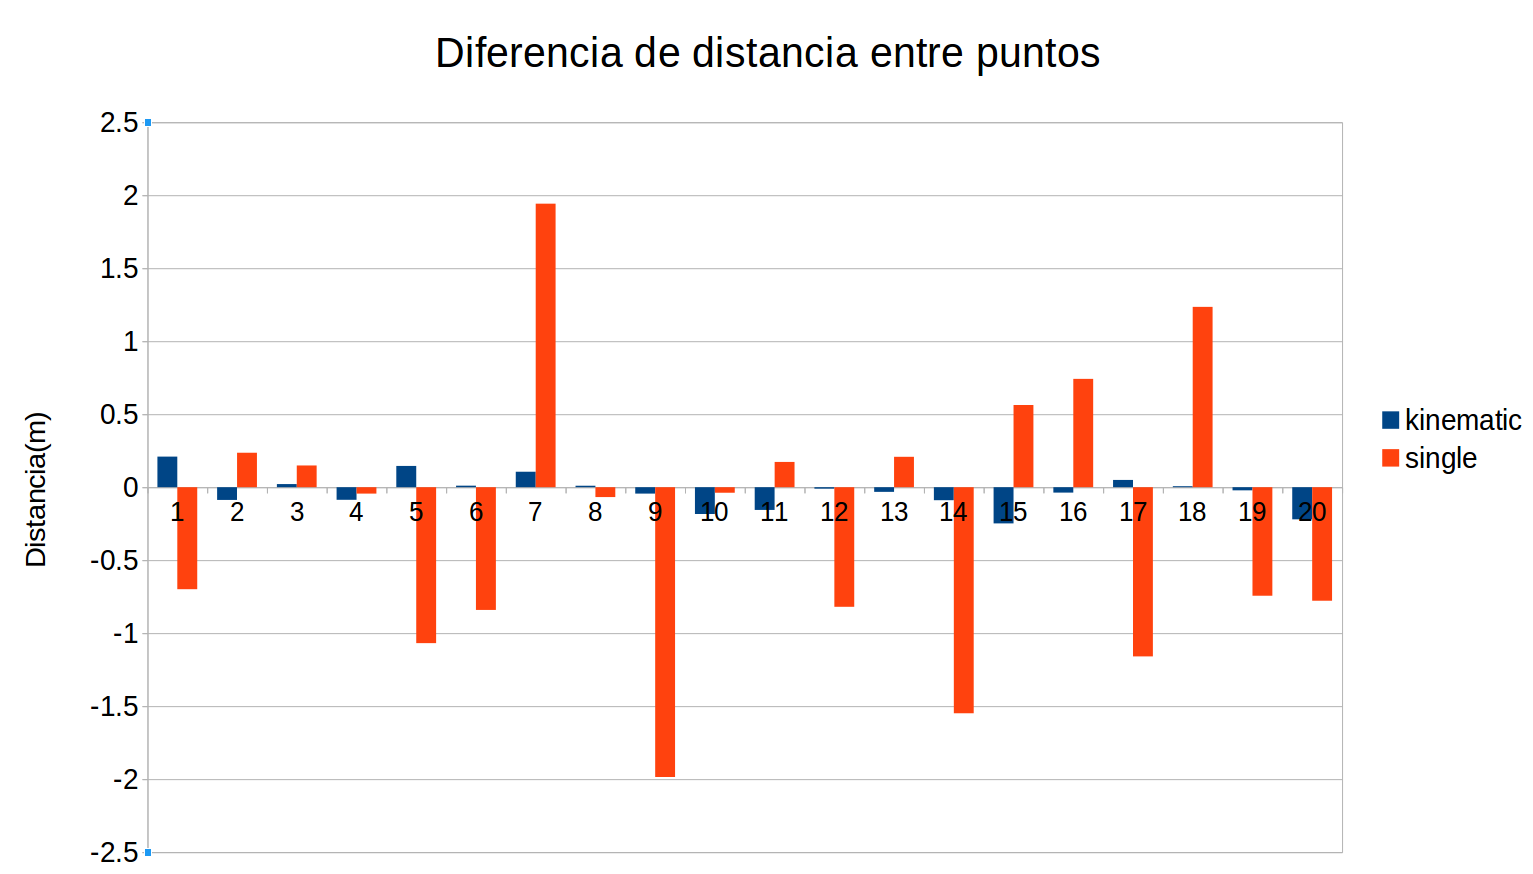
\includegraphics[width=0.95\textwidth]{Figures/ErrMts}
\caption[Diferencia entre la distancia medida entre puntos y la distancia nominal de 3 metros por segmento.]{Diferencia entre la distancia medida entre puntos y la distancia nominal de 3 metros por segmento.}
\label{fig:ErrMts}
\end{figure}

El error promedio obtenido en ambas modalidades se muestra en la figura~\ref{fig:ErrProm}. En modo \textbf{Real-Time Kinematics}, se obtuvo un error promedio de \textbf{$\pm 0.08876$} metros, en contraste al modo sin retroalimentación o \textbf{Single}, donde se obtuvo un error promedio de \textbf{$\pm 0.752035$} metros.

\begin{figure}[H]
\centering
\includegraphics[width=0.95\textwidth]{Figures/ErrProm}
\caption[Diferencia entre la distancia medida entre puntos y la distancia nominal de 3 metros por segmento.]{Diferencia entre la distancia medida entre puntos y la distancia nominal de 3 metros por segmento.}
\label{fig:ErrProm}
\end{figure}

Finalmente, las coordenadas obtenidas durante la rutina se muestran en el mapa en las figuras~\ref{fig:NoRtkRes}~y~\ref{fig:RtkRes}, siendo la primera la solución sin retroalimentación y la segunda la solución con RTK.

\begin{figure}[H]
\centering
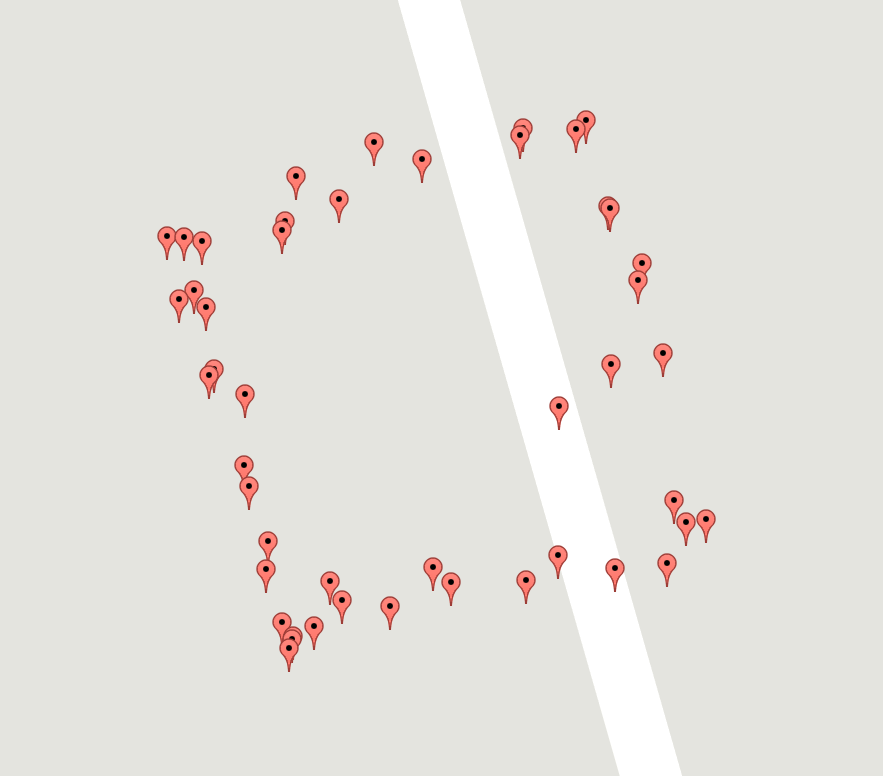
\includegraphics[width=0.8\textwidth]{Figures/NoRtkRes}
\caption[Muestras obtenidas sin Real-Time Kinematics.]{Muestras obtenidas por el sistema sin Real-Time Kinematics.}
\label{fig:NoRtkRes}
\end{figure}

\begin{figure}[H]
\centering
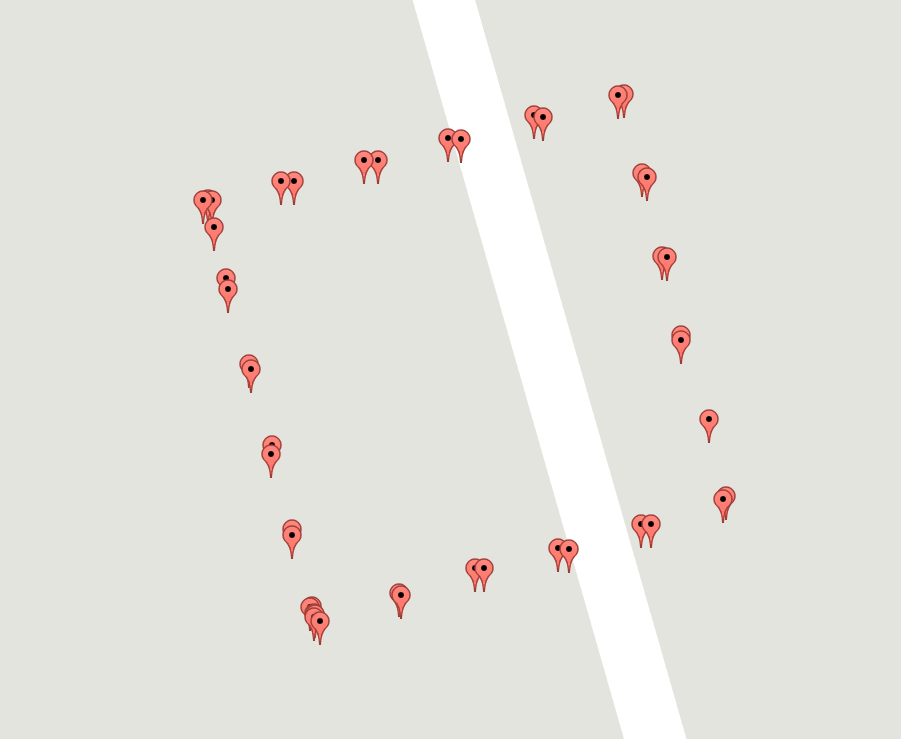
\includegraphics[width=0.8\textwidth]{Figures/RtkRes}
\caption[Muestras obtenidas por el sistema con Real-Time Kinematics.]{Muestras obtenidas por el sistema \textbf{con Real-Time Kinematics}.}
\label{fig:RtkRes}
\end{figure}

Nótese cómo en la solución sin retroalimentación (figura~\ref{fig:NoRtkRes}) se muestran variaciones muy altas en las líneas rectas que conforman el cuadrado, y las muestras se ven afectadas notoriamente en el lado este de la figura. Por otro lado, en la solución con RTK se muestra un mucho mejor ajuste a los puntos marcados y se observa un mejor acoplamiento a la forma del cuadrado.

\section{Conclusión}
Tras el análisis de los resultados, se determinó que la solución con Real-Time Kinematics ayuda a mantener la estabilidad de las mediciones de GPS, siendo 8.47 veces más precisa que la solución Single, pudiendo determinar mejor la posición de los puntos al realizar un recorrido de una rutina previamente estructurada. 
% Chapter 2

\chapter{Conclusiones} % Main chapter title

\label{Conc} % For referencing the chapter elsewhere, use \ref{Chapter2} 

Pepe 

%----------------------------------------------------------------------------------------
%	THESIS CONTENT - APPENDICES
%----------------------------------------------------------------------------------------

\appendix % Cue to tell LaTeX that the following "chapters" are Appendices
\label{Chap:Anexos}
% Include the appendices of the thesis as separate files from the Appendices folder
% Uncomment the lines as you write the Appendices

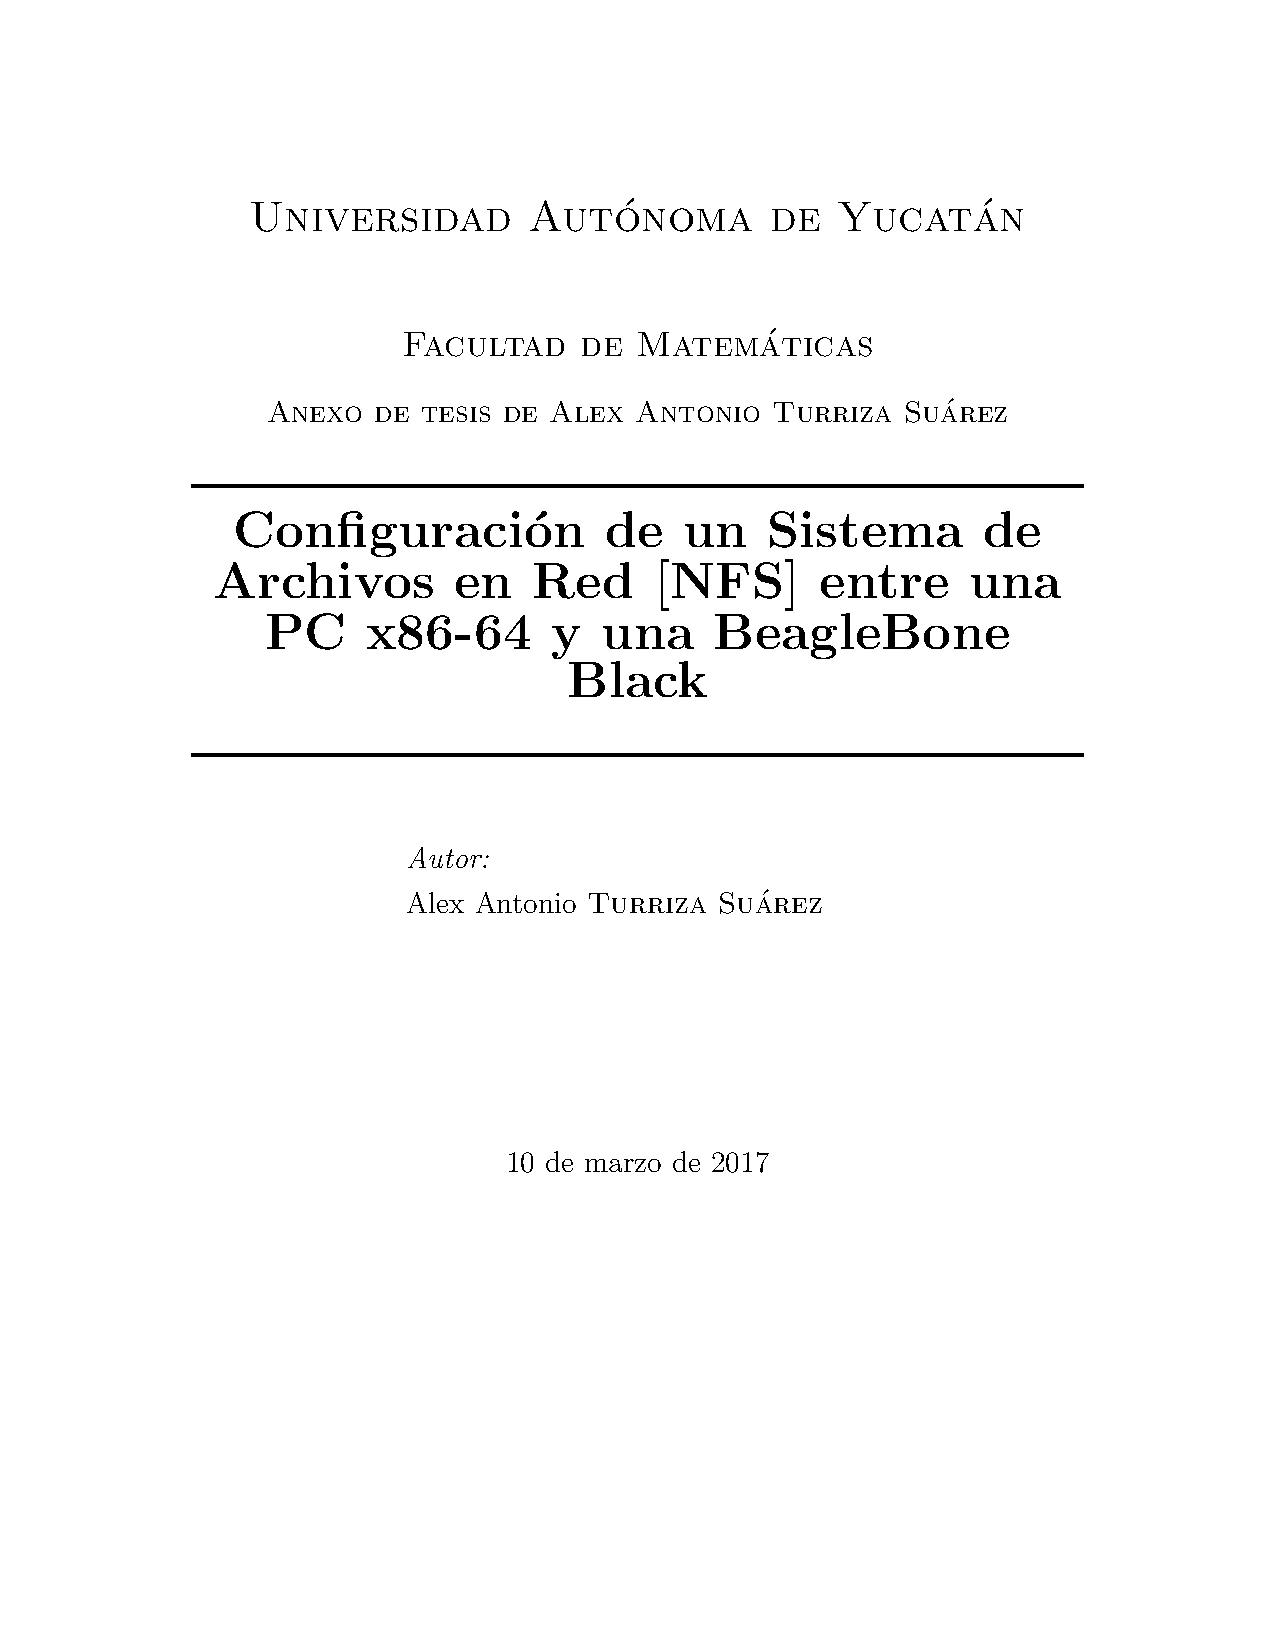
\includepdf[pages=-]{Apendices/nfs}
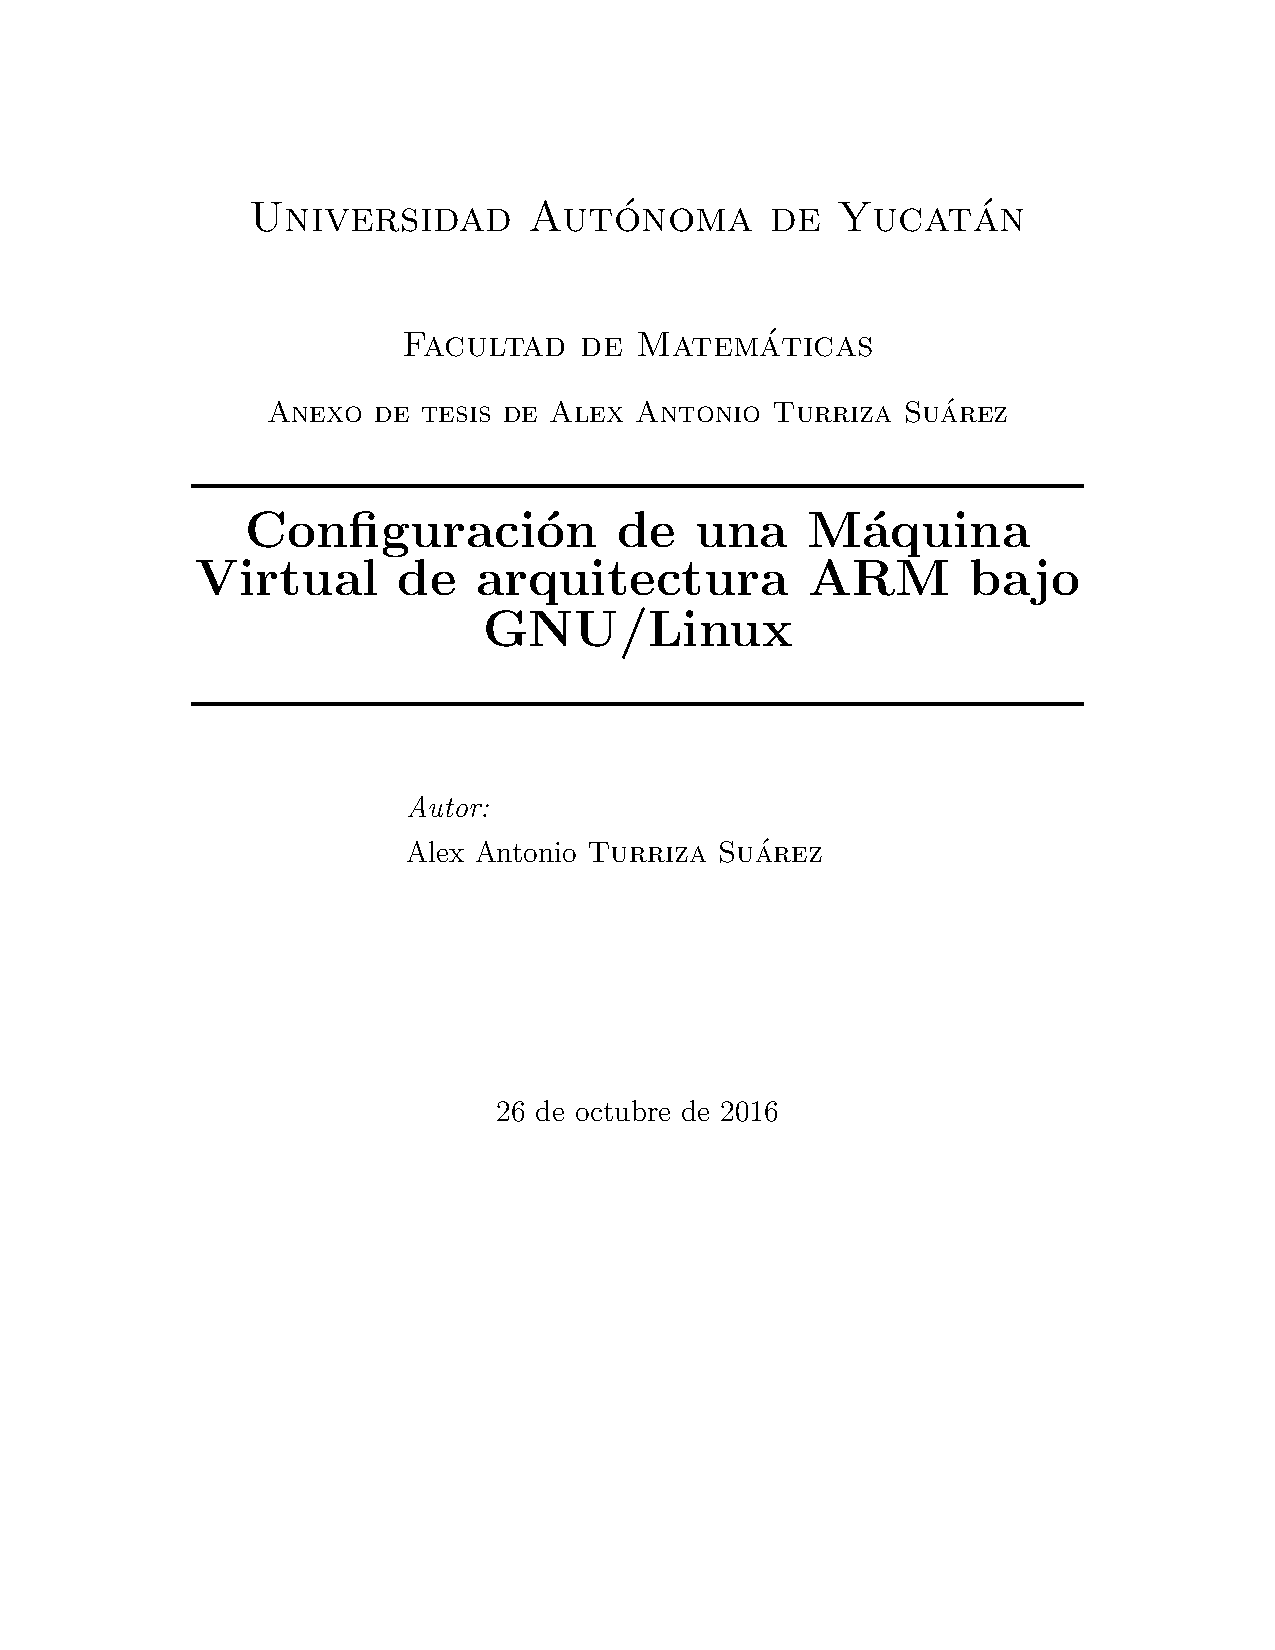
\includepdf[pages=-]{Apendices/qemu}
\includepdf[pages=-]{Apendices/xbeeGuia}

%%%%%%%%%%%%%%%%%%%%%%%%%%%%%%%%%%%%%%%%%%
% Simple Sectioned Essay Template
% LaTeX Template
%
% This template has been downloaded from:
% http://www.latextemplates.com
%
% Note:
% The \lipsum[#] commands throughout this template generate dummy text
% to fill the template out. These commands should all be removed when 
% writing essay content.
%
%%%%%%%%%%%%%%%%%%%%%%%%%%%%%%%%%%%%%%%%%

%----------------------------------------------------------------------------------------
%	PACKAGES AND OTHER DOCUMENT CONFIGURATIONS
%----------------------------------------------------------------------------------------

%\documentclass[12pt]{article} % Default font size is 12pt, it can be changed here

%\usepackage{geometry} % Required to change the page size to A4
%\geometry{letterpaper} % Set the page size to be A4 as opposed to the default US Letter

%\usepackage{graphicx} % Required for including pictures

%\usepackage{listings} %Para comandos bash Linux

%\usepackage{float} % Allows putting an [H] in \begin{figure} to specify the exact location of the figure
%\usepackage{wrapfig} % Allows in-line images such as the example fish picture

%\usepackage{color} %textos de colores

%\usepackage[spanish]{babel}

%\usepackage[utf8]{inputenc} %Uso de acentos directamente

%\usepackage{hyperref}

%\linespread{1.2} % Line spacing

%\setlength\parindent{0pt} % Uncomment to remove all indentation from paragraphsre

%\graphicspath{{Pictures/}} % Specifies the directory where pictures are stored

%\begin{document}

%----------------------------------------------------------------------------------------
%	TITLE PAGE
%----------------------------------------------------------------------------------------

%\begin{titlepage}

%\newcommand{\HRule}{\rule{\linewidth}{0.5mm}} % Defines a new command for the horizontal lines, change thickness here

%\center % Center everything on the page

%\textsc{\LARGE Universidad Autónoma de Yucatán}\\[1.5cm] % Name of your university/college
%\textsc{\Large Facultad de Matemáticas}\\[0.5cm] % Major heading such as course name
%\textsc{\large Anexo de tesis de Alex Antonio Turriza Suárez}\\[0.5cm] % Minor heading such as course title

%\HRule \\[0.4cm]
%{ \huge \bfseries Configuración de un Sistema de Archivos en Red [NFS] entre una PC x86-64 y una BeagleBone Black}\\[0.4cm] % Title of your document
%\HRule \\[1.5cm]
%\begin{minipage}{0.5\textwidth}
%\begin{flushleft} \large
%\emph{Autor:}\\
%Alex Antonio \textsc{Turriza Suárez} % Your name
%\end{flushleft}
%\end{minipage}
%~
%\begin{minipage}{0.4\textwidth}
%\begin{flushright} \large
%\emph{Asesores:} \\
%Dr. Arturo \textsc{Espinosa Romero} \\
%\ \ \\
%Dr. Anabel \textsc{Martín González}
%\end{flushright}
%\end{minipage}\\[4cm]

%{\large \today}\\[3cm] % Date, change the \today to a set date if you want to be precise

%\includegraphics{Logo}\\[1cm] % Include a department/university logo - this will require the graphicx package

%\vfill % Fill the rest of the page with whitespace

%\end{titlepage}

%----------------------------------------------------------------------------------------
%	TABLE OF CONTENTS
%----------------------------------------------------------------------------------------

%\tableofcontents % Include a table of contents

%\newpage % Begins the essay on a new page instead of on the same page as the table of contents 

%----------------------------------------------------------------------------------------
%	INTRODUCTION
%----------------------------------------------------------------------------------------
\chapter{Sistema de Archivos en Red entre una PC y una BeagleBone Black}\label{Anx:nfs}
\section{Introducción}
Cuando dos máquinas de diferente arquitectura deben trabajar en un sólo proyecto, suele suceder que es mucho más cómodo realizar código y documentación en una, a pesar de que que los archivos estén destinados a ser usados en la otra.

Para ello, se mostrará la forma de configurar un sistema de archivos en red NFS que facilite la tarea de compartir archivos en un directorio.

En este trabajo se mostrará la instalación del sistema en una máquina host en una PC y un cliente en una BeagleBone Black, aprovechando que al conectar mediante USB, se crea una red entre ambas plataformas.

%------------------------------------------------

\section{Definición de NFS}
Sistema de archivos en red (NFS, "\textit{Network File System}" por sus siglas en inglés), es un protocolo que permite acceder mediante una conexión remota a un sistema de archivos [\href{https://debian-handbook.info/browse/es-ES/stable/sect.nfs-file-server.html}{El Manual del Administrador de Debian}\footnotemark, consultado en Octubre 2016].

\footnotetext{\href{https://debian-handbook.info/browse/es-ES/stable/sect.nfs-file-server.html}{https://debian-handbook.info/browse/es-ES/stable/sect.nfs-file-server.html}}

En su funcionamiento, permite que un equipo host comparta determinado directorio con otros equipos clientes, pudiendo determinar qué equipos tienen permisos de lectura, escritura o ambas.

%------------------------------------------------

\section{Descarga e instalación}\label{sec:_install} % Sub-section

\subsection{Instalación en host / PC}
Bajo Ubuntu en sus últimas versiones en el momento de la redacción de éste documento, se abre una terminal con los comandos \textit{Ctrl + Alt + t}.

Lo primero, es actualizar los repositorios con:
\begin{lstlisting}[language=bash]
$ sudo apt-get update
\end{lstlisting}

Una vez actualizados, se procede a la instalación de un paquete mediante el siguiente comando:

\begin{lstlisting}[language=bash]
$ sudo apt-get install nfs-kernel-server 
\end{lstlisting}

Al finalizar la descarga e instalación, se debe modificar un archivo. Copiar en la terminal el siguiente comando y colocar la contraseña:
\begin{lstlisting}[language=bash]
$ sudo nano /etc/default/nfs-kernel-server
\end{lstlisting}

Se debe modificar la línea \textbf{NEED\_SVCGSSD=""} y colocar $"no"$ en el entrecomillado, como muestra la figura \ref{fig:NFSKer}. Cuando se termine de modificar, guardar con la combinación de teclas $Ctrl + O$ y regresar a la terminal con $Ctrl + X$.

\begin{figure}[H] % Example image
\center{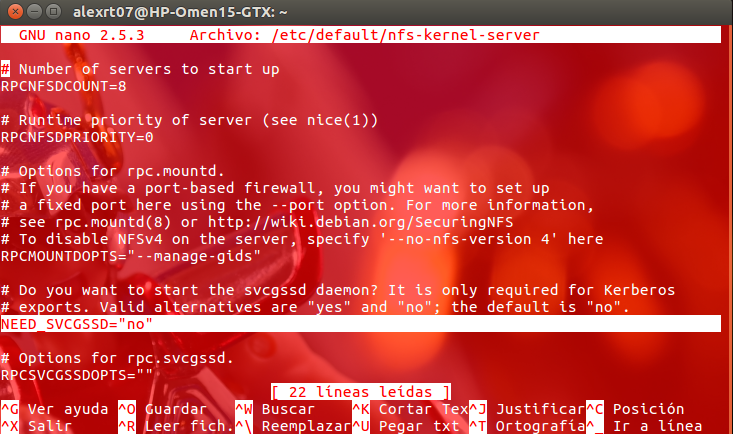
\includegraphics[width=0.9\linewidth]{Figures/NFS/NFS1}}
\caption{Archivo /etc/default/nfs-kernel-server ya modificado.}
\label{fig:NFSKer}
\end{figure}

Lo siguiente es abrir el archivo ubicado en /etc/idmapd.conf:
\begin{lstlisting}[language=bash]
$ sudo nano /etc/idmapd.conf 
\end{lstlisting}

Verificar que existan las líneas $Nobody-User = nobody$ y $Nobody-Group = nogroup$ como muestra la figura \ref{fig:NFSKer2}.

\begin{figure}[H] % Example image
\center{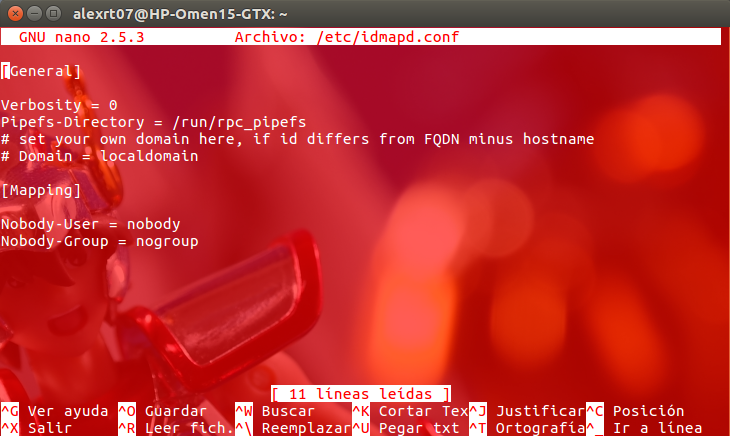
\includegraphics[width=0.9\linewidth]{Figures/NFS/NFS2}}
\caption{Archivo /etc/idmapd.conf.}
\label{fig:NFSKer2}
\end{figure}

Cuando se realiza una conexión con la BeagleBone Black mediante un cable USB, se crea una red con las siguientes direcciones: $192.168.7.2$ para la BeagleBone y $192.168.7.1$ para el PC host. Entonces, tomando en cuenta lo anterior, se modifica el archivo /etc/exports de la siguiente manera:

Se abre el archivo con nano, en la terminal:

\begin{lstlisting}[language=bash]
$ sudo nano /etc/exports
\end{lstlisting}

En el archivo que se abre, añadir la siguiente línea (note que dentro del paréntesis, entre los comandos no existen espacios):

\begin{lstlisting}[language=bash]
/home/alexrt07/Escritorio/Alex     192.168.7.2(rw,sync,
no_root_squash,no_subtree_check)
\end{lstlisting}

Donde /home/alexrt07/Escritorio/Alex es el directorio a compartir y 192.168.7.2 es la dirección ip de la BeagleBone. Así, el archivo queda como muestra la figura \ref{fig:NFSKer3}.

\begin{figure}[H] % Example image
\center{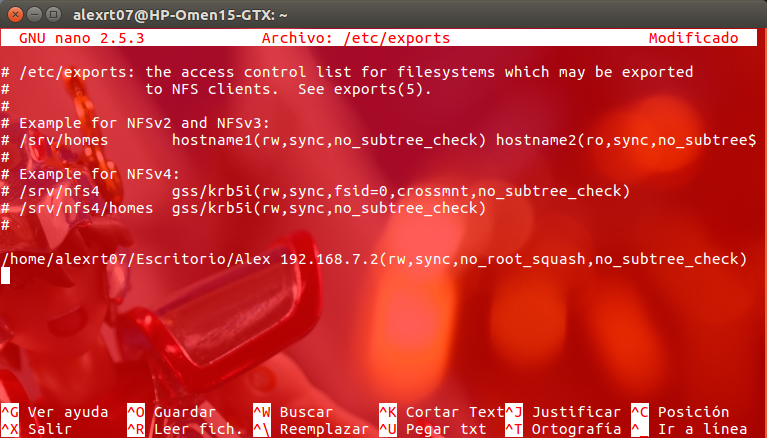
\includegraphics[width=0.9\linewidth]{Figures/NFS/NFS3}}
\caption{Archivo /etc/exports.}
\label{fig:NFSKer3}
\end{figure}

Finalmente, resta reiniciar el servidor con el siguiente comando: 

\begin{lstlisting}[language=bash]
$ /etc/init.d/nfs-kernel-server restart
\end{lstlisting}

Se deberá mostrar una confirmación de reinicio exitoso.
%---------------------------------------------------

\subsubsection{Seguridad}\label{subsec:conf}

Para evitar dejar hoyos de seguridad de acceso a los archivos personales, es altamente recomendable modificar los archivos /etc/hosts.deny y /etc/hosts.allow para permitir acceso solamente a los clientes conocidos.

Abrir el archivo /etc/hosts.deny con:

\begin{lstlisting}[language=bash]
$ sudo nano /etc/hosts.deny
\end{lstlisting}

Y añadir la siguiente línea:

\begin{lstlisting}[language=bash]
rpcbind mountd nfsd statd lockd rquotad : ALL
\end{lstlisting}

\begin{figure}[H] % Example image
\center{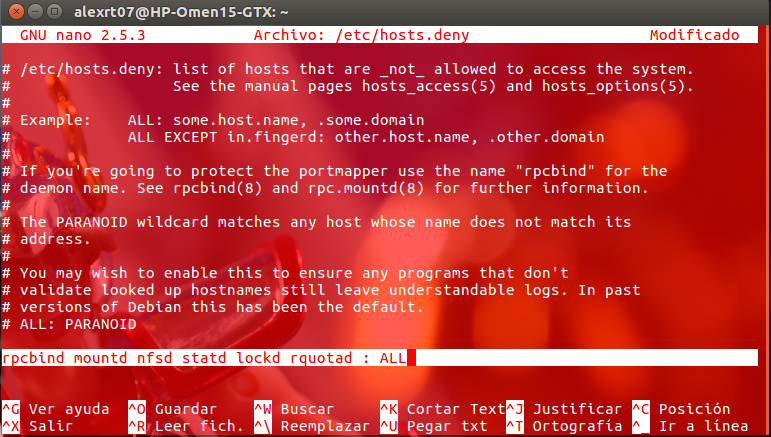
\includegraphics[width=0.9\linewidth]{Figures/NFS/NFS4}}
\caption{Archivo /etc/hosts.deny}
\label{fig:NFSKer4}
\end{figure}

Como muestra la figura \ref{fig:NFSKer4}. Ahora, abrir el archivo /etc/hosts.allow con el comando:

\begin{lstlisting}[language=bash]
$ sudo nano /etc/hosts.allow
\end{lstlisting}

Y añadir la siguiente línea:

\begin{lstlisting}[language=bash]
  rpcbind mountd nfsd statd lockd 
  rquotad : 192.168.7.2 127.0.0.1 
\end{lstlisting}

Como muestra la figura \ref{fig:NFSKer5}.

\begin{figure}[H] % Example image
\center{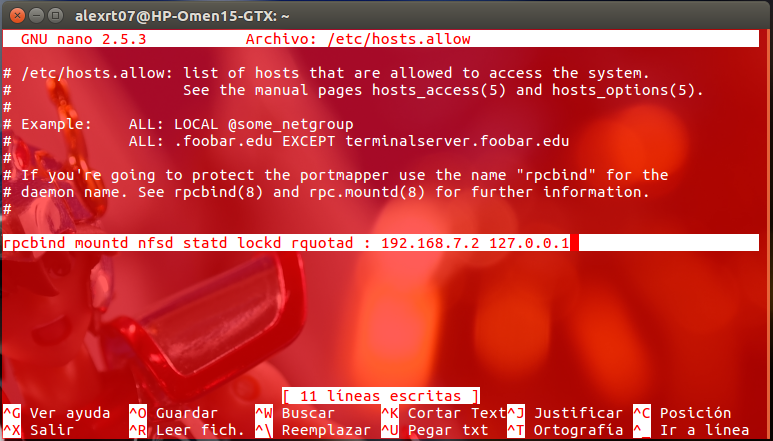
\includegraphics[width=0.9\linewidth]{Figures/NFS/NFS5}}
\caption{Archivo /etc/hosts.allow}
\label{fig:NFSKer5}
\end{figure}

Reiniciar el servidor con: 

\begin{lstlisting}[language=bash]
$ service nfs-kernel-server restart
\end{lstlisting}

Ahora, el PC está preparado para compartir vía red el directorio:

\begin{lstlisting}[language=bash]
/home/alexrt07/Escritorio/Alex/
\end{lstlisting}

\subsection{Instalación en cliente / BeagleBone}

Asumiendo que la BeagleBone Black tiene un Debian con su archivo \textit{/etc/apt/sources.list} correctamente configurado, ejecutamos en la terminal de nuestro host para conectarnos:

\begin{lstlisting}[language=bash]
$ ssh -l root 192.168.7.2
\end{lstlisting}

donde \textit{ssh} es el comando para conectarse por el protocolo secure shell, \textit{-l} es el comando que indica que se hará un login con el usuario \textit{root}, y \textit{192.168.7.2} es la dirección IP de la BeagleBone en la red que se creó a través del cable USB.

Entonces, una vez hecho el loggin, ejecutar:

\begin{lstlisting}[language=bash]
$ apt-get install nfs-common
\end{lstlisting}

Que instalará y preconfigurará los archivos necesarios para una correcta comunicación a través de NFS.

Es recomendable crear un directorio en donde se montarán los archivos que compartirá con la PC:

\begin{lstlisting}[language=bash]
$ mkdir /home/debian/Alex_tesista
\end{lstlisting}

\section{Ejecución}

Se procede a montar el sistema de archivos con el siguiente comando:

\begin{lstlisting}[language=bash]
$ mount -t nfs -o proto=tcp,port=2049 
  192.168.7.1:/home/alexrt07/ARM-Root/home/Alex 
  /home/debian/Alex_tesista/
\end{lstlisting}

En donde \textit{mount} es el comando para montar el directorio, \textit{-t nfs} indica que se trata de un sistema de archivos por red, \textit{-o proto=tcp,port=2049} indica que se utilizará el protocolo de transferencia de archivos a través del puerto 2049 (mirar el manual de nfs en su página 5 con \textbf{\$ man 5 nfs} para más opciones e información),\textit{192.168.7.1:} es la dirección IP de la PC host, \textit{/home/alexrt07/ARM-Root/home/Alex} es el directorio que contiene los archivos a compartir, y \textit{/home/debian/Alex\_tesista/} es el directorio creado en donde se encontrarán los archivos.

Para cerrar esta conexión, utilice

\begin{lstlisting}[language=bash]
$ umount /home/debian/Alex_tesista/
\end{lstlisting}

Tome en cuenta que al finalizar la conexión, no se mantendrán los archivos compartidos por nfs. Desaparecerán y contendrá los archivos originales que esa carpeta contenía antes de montar el sistema de archivos por red.

%\end{document}
%\include{Appendices/AppendixB}
%\include{Appendices/AppendixC}

%----------------------------------------------------------------------------------------
%	BIBLIOGRAPHY
%----------------------------------------------------------------------------------------

%\printbibliography[heading=bibintoc]
\printbibliography

%----------------------------------------------------------------------------------------

\end{document}  
